% Nanyang Technological University - Qualification Examination report template
% 1st Draft 27/June/2014 (v.1.0) (Written by Ali Qasim - eng.amq@gmail.com)
% A modified version of Harvard thesis template
% ---------------------------------------------------------------------------- %
% Update v.1.1 26/August/2014 (Written by Ali Qasim - eng.amq@gmail.com)
% 1- Abstract moved to the beginning of the frontmatter.
% 2- Page numbering format for frontmatter changed to capitalized roman "Roman".
% 3- Cover page is a closer match to that provided by the faculty, with an empty page added after it.
% 4- Modified IEEE citation style to disable replacing author names with dashes in consecutive references with similar author names.

% ---------------------------------------------------------------------------- %
% Set Document Class
% ---------------------------------------------------------------------------- %
\documentclass[11pt,oneside,final]{ntu_qe}

\newcommand{\numcol}{1}
% ---------------------------------------------------------------------------- %
% Includes Packages
% ---------------------------------------------------------------------------- %

%-----------------------------------------------------------
% Customized
\usepackage[utf8]{vietnam}
%\usepackage{breqn}
\usepackage{enumitem}
\usepackage{amsmath}
\usepackage{mathrsfs}
\usepackage{mathtools}

\usepackage{listings}
\usepackage{xcolor}
\usepackage{bbm}


%\usepackage[style=authoryear,backend=biber]{biblatex}
%\usepackage{mathptmx}

\definecolor{codegreen}{rgb}{0,0.6,0}
\definecolor{codegray}{rgb}{0.5,0.5,0.5}
\definecolor{codepurple}{rgb}{0.58,0,0.82}
\definecolor{backcolour}{rgb}{0.95,0.95,0.92}

\lstdefinestyle{mystyle}{
	backgroundcolor=\color{backcolour},   
	commentstyle=\color{codegreen},
	keywordstyle=\color{magenta},
	numberstyle=\tiny\color{codegray},
	stringstyle=\color{codepurple},
	basicstyle=\ttfamily\footnotesize,
	breakatwhitespace=false,         
	breaklines=true,                 
	captionpos=b,                    
	keepspaces=true,                 
	numbers=left,                    
	numbersep=5pt,                  
	showspaces=false,                
	showstringspaces=false,
	showtabs=false,                  
	tabsize=2
}

\lstset{style=mystyle}

%%%%%%%%%%%%%%%%%%%%%%%%%%%%%%%%%%%%%%%%%%%%%%%%%%%%%%%%%%%%%%%%

\let\proof\relax
\let\endproof\relax
\usepackage{amsthm}
%-----------------------------------------------------------


\usepackage{NTUdis}
\usepackage{setspace}
\usepackage{graphicx} 
\graphicspath{{Figures/}}
\usepackage{float}
\usepackage{subfigure}
%\usepackage{algorithm}
\usepackage{amsfonts}
\usepackage{ifthen}
\usepackage{booktabs}
\usepackage{amssymb}
\usepackage{supertabular}
\usepackage{array}
\usepackage{multirow}
\usepackage{fancyhdr}
%\usepackage{fancyheadings}
\usepackage{psfrag}
\usepackage{amsmath}
\usepackage{hhline}
\usepackage{type1cm}
\usepackage{lettrine}
\usepackage{cite}
\usepackage{fancybox}
\usepackage{ctable}

\usepackage[ruled,vlined]{algorithm2e}
% ---------------------------------------------------------------------------- %
% Document Setting
% ---------------------------------------------------------------------------- %
% Front Matters
% Labels : 1) All labels starts with fig, table, algo, eqn
% 2) use relative directory. current file name. name 
% fig:wdcdf.thesis.algo.tex.flow_chart
%

% define the following before \input this tex
% \newcommand{\numcol}{2}
\newcommand{\checkOneCol}{\ifthenelse{\numcol = 1}}

\newcommand{\tablefont}{\small}

% Wrapping functions 
\newcommand{\wchapter}{\chapter}
\newcommand{\wsection}{\section}
\newcommand{\wsubsection}{\subsection}
\newcommand{\wsubsubsection}{\subsubsection}

% -- abstract
\newcommand{\wabstract} {\begin{abstract}}
\newcommand{\wendabstract} {\end{abstract}}

% -- mathematics
\newcommand{\weqnarray}{\begin{eqnarray}}
\newcommand{\wendeqnarray} {\end{eqnarray}}
\newcommand{\waligneqnarray}{\begin{align}}
\newcommand{\walignendeqnarray} {\end{align}}

% -- lines
\newcommand{\emptyline}{\noindent\newline}
\newcommand{\emptyindentline}{\emptyline\indent}

% -- table
\newcommand{\wtable}{\begin{table}}
\newcommand{\wendtable}{\end{table}}

% -- figure
\newcommand{\wfigure}{\begin{figure}}
\newcommand{\wendfigure}{\end{figure}}

% -- list
\newcommand{\wlist}{\begin{itemize}}
\newcommand{\wendlist}{\end{itemize}}
\newcommand{\wdesc}{\begin{description}}
\newcommand{\wenddesc}{\end{description}}

% -- Number List
\newcommand{\wnumlist}{\begin{enumerate}}
\newcommand{\wendnumlist}{\end{enumerate}}

% String declaration for references
\newcommand{\lfig}{Fig.}
\newcommand{\ltable}{Table}
\newcommand{\lalgo}{Algorithm}
\newcommand{\leqn}{Eqn.}
\newcommand{\llemma}{Lemma}
\newcommand{\lcorollary}{Corollary}
\newcommand{\ltheorem}{Theorem}
\newcommand{\ldef}{Def.}
\newcommand{\lsection}{Section}
\newcommand{\lchapter}{Chapter}
\newcommand{\lappendix}{Appendix}
\newcommand{\lexample}{Example}
\newcommand{\lcase}{Case}
%
% Format for mathematics
%\newtheorem{theorem}{Theorem}
\newtheorem{theorem}{Định lý}[section]
\newtheorem{lemma}{Lemma}
\newtheorem{corollary}{Corollary}
%\newtheorem{definition}{Definition}
\newtheorem{definition}{Định nghĩa}[section]
\newtheorem{example} {Example}
\newtheorem{case} {Case}

\makeatletter
\renewcommand{\@chapapp}{Chương}
\makeatother

\newtheorem{exercise}{Bài tập}[chapter]
%\newtheorem{exercise}{Bài tập}[section]
\theoremstyle{definition}
\newtheorem*{solution}{Bài giải}
\newtheorem*{proofs}{Chứng minh}


%
\newcommand{\wtheorem}{\begin{theorem}}
\newcommand{\wendtheorem}{\end{theorem}}
\newcommand{\wlemma}{\begin{lemma}}
\newcommand{\wendlemma}{\end{lemma}}
\newcommand{\wcorollary}{\begin{corollary}}
\newcommand{\wendcorollary}{\end{corollary}}
\newcommand{\wdefinition}{\begin{definition}}
\newcommand{\wenddefinition}{\end{definition}}
\newcommand{\wexample}{\begin{example}}
\newcommand{\wendexample}{\end{example}}
\newcommand{\wproof}{\begin{proof}}
\newcommand{\wendproof}{\end{proof}}
\newcommand{\wcase}{\begin{case}}
\newcommand{\wendcase}{\end{case}}
%\renewcommand{\QED}{\QEDopen}
%

\DeclareMathOperator{\sub}{sub}
\DeclareMathOperator{\im}{Im}
\DeclareMathOperator{\Ker}{Ker}
\DeclareMathOperator{\rank}{rank}
\DeclareMathOperator*{\argmax}{arg\,max}
\DeclareMathOperator*{\argmin}{arg\,min}
\newcommand{\normiii}[1]{{\left\vert\kern-0.25ex\left\vert\kern	-0.25ex\left\vert #1 
		\right\vert\kern-0.25ex\right\vert\kern-0.25ex\right\vert}}
% - Spacing mode
\newcommand{\setsinglespace}{\ssp}
\newcommand{\setonehalfspace}{\hsp}
\newcommand{\setdoublespace}{\dsp}
% - Define the function "NewPage" to force create a new page when needed
\newcommand*\NewPage{\newpage\null\thispagestyle{empty}\newpage}
% ---------------------------------------------------------------------------- %
% Table Of Contents Setup
% - max depth listed:
% 1 = section, 2 = subsection, 3 = subsubsection
% ---------------------------------------------------------------------------- %

%
% HaQT
\newcommand{\smallwedge}{\scriptscriptstyle \wedge} 
%

\setcounter{tocdepth}{3}

\begin{document}
\setdoublespace
% ---------------------------------------------------------------------------- %
% Title page
% includes -  Front and Second covers
% ---------------------------------------------------------------------------- %
%\pagestyle{empty}

% ----------------------------------------------------------------------------
% Title Page
% ----------------------------------------------------------------------------
%\university{Đại học Khoa học Tự nhiên}
\title{Title}
\author{Author}
\degreemonth{Tháng 4,} % month final submission occurs.
\degreeyear{2021}
\field{Electrical Engineering}
\department{Trường Đại học Khoa học Tự nhiên Hà Nội}
%\school{Nanyang Technological University}
%\advisor{Associate Professor Dr. Ali Nagaratnam Zhang}
\degreetype{Tiểu luận khoa học}
%\matricno{Matric Number}
\matricno{}
\maketitle
%\copyrightpage
\hsp
\NewPage
% ---------------------------------------------------------------------------- %
% Front Matters
% includes - Table of Contents, Abstract, Acknowledgement, 
% List of Figures and List of Tables
% ---------------------------------------------------------------------------- %
%% ---------------------------------------------------------------------------- %
% Front Matters
% ---------------------------------------------------------------------------- %
% ---------------------------------------------------------------------------- %
% Acknowledgement
% ---------------------------------------------------------------------------- %
% ---------------------------------------------------------------------------- %
% Abstract
% ---------------------------------------------------------------------------- %

%\setsinglespace
%\begin{nabstract}
%% ----------------------------------------------------------------------------
% Abstract
% ----------------------------------------------------------------------------
\indent Abstract text here..
%\newpage
%\end{nabstract}

\setonehalfspace
%\addcontentsline{toc}{section}{Table of Contents}
\addcontentsline{toc}{section}{Mục lục}
\tableofcontents
%\listoffigures
%\listoftables

\newpage
\startarabicpagination
%END

%\setdoublespace
% ---------------------------------------------------------------------------- %
\hsp
% ---------------------------------------------------------------------------- %
% Chapter 0 - 
\chapter*{Lời nói đầu}\label{CH3}
\par Xử lý tín hiệu là một đề tài đóng vai trò rất quan trọng trong các ngành kĩ thuật. Tín hiệu mà chúng ta thu được có thể là âm thanh, hình ảnh,... Âm thanh là kết quả của sự dao động trong màng nhĩ lỗ tai, được mô phỏng bằng sóng âm lan truyền trong không khí phát ra từ tai nghe, âm thanh nhạc cụ, tiếng nói của con người,... Khi vẽ đồ thị những dao động này theo cường độ hay áp suất theo thời gian, ta được biểu diễn hình ảnh của âm thanh. Bên cạnh đó, tín hiệu biểu diễn cho hình ảnh là một hàm biến đổi, tuy nhiên, hàm biến đổi này không biến đổi theo thời gian mà biến đổi theo không gian hai chiều của ảnh. Về cơ bản có thể chia thành hai loại tín hiệu đó là tín hiệu liên tục và tín hiệu rời rạc. 
\par Để xử lý tín hiệu, chúng ta có nhiều phương pháp biến đổi tín hiệu nhằm biểu diễn dưới các miền không gian khác nhau như biến đổi Cosine, biến đổi Wavelet,... và không thể không kể đến biến đổi Fourier. Phương pháp biến đổi Fourier được đặt dựa theo tên của nhà toán học người Pháp Joseph Fourier, thực hiện việc biến đổi tín hiệu từ miền thời gian (chủ yếu là tín hiệu liên tục), hoặc miền không gian (chủ yếu là tín hiệu rời rạc) sang miền tần số. Biến đổi Fourier được sử dụng khi muốn sử dụng các đặc điểm hình học của một tín hiệu trong miền không gian vì tín hiệu trong miền tần số được phân rã thành các thành phần hình sin của nó, nên rất dễ kiểm tra hoặc xử lý các tần số nhất định, từ đó gây ra ảnh hưởng đến cấu trúc hình học trong miền không gian.
\par Trên cơ sở đó, nội dung đồ án của em gồm ba chương:
\begin{itemize}
    \item Chương 1 trình bày về kiến thức cơ sở. Tìm hiểu về phép biến đổi Fourier (nguồn gốc, xuất xứ,...), các tính chất và đặc điểm nói chung về mặt toán học và nói riêng về lĩnh vực xử lý ảnh số. Giới thiệu tổng quan về sự phát triển của các ứng dụng dùng phép biến đổi Fourier trong xử lý ảnh theo thời gian.
    \item Chương 2 trình này một số ứng dụng của biến đổi Fourier và lập trình bằng ngôn ngữ MATLAB trên các kiểu ảnh số khác nhau như ảnh màu, ảnh cấp xám, ảnh y tế,...
    \item Chương 3 trình bày một ứng dụng biến đổi Fourier trong nén ảnh số được đưa ra trong bài báo [25] của các tác giả Mohammed H. Rasheed và đồng nghiệp công bố năm 2020.
\end{itemize}

% ---------------------------------------------------------------------------- %
% Chapter 1
\chapter{Kiến thức cơ sở}\label{CH1}
\section{Giới thiệu}
\par Tín hiệu (hàm số) dù liên tục hay rời rạc thì ở trong các miền không gian khác nhau sẽ mang những đặc trưng khác nhau. Chẳng hạn ta có đồ thị của các hàm số trong miền không gian khác nhau như trong hình 1.1.

\begin{center}
    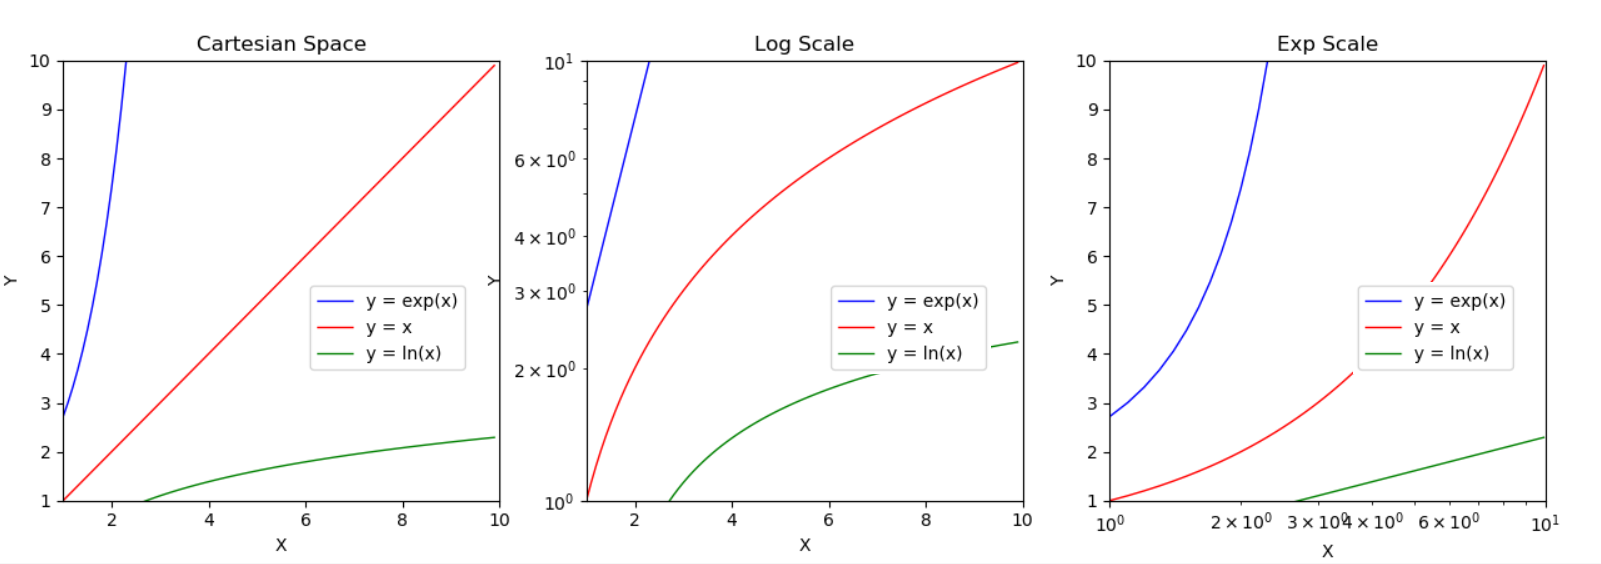
\includegraphics[scale=0.4]{Figures/diff_space.png}
    \par \textbf {Hình 1.1} Đồ thị hàm số trong các miền không gian khác nhau.
\end{center}
Đồ thị của hàm số $y=x$ trong miền không gian Cartesian có dạng đường thẳng, nhưng trong miền không gian mũ lại có dạng đường cong parabol, hoặc đồ thị hàm số $y=e^x$ có dạng parabol trong không gian Cartesian thông thường lại có dạng đường thẳng trong không gian logarit tự nhiên. Giá trị, số lượng các thông tin vẫn được bảo tồn và có thể thực hiện biến đổi qua lại giữa các miền không gian. Như vậy, việc khai thác đặc trưng các tín hiệu trong đa dạng các miền không gian sẽ mang lại những hiệu quả nhất định.
\par Có nhiều phép biến đổi tín hiệu sang các miền không gian khác nhau như biến đổi Cosine, biến đổi Fourier, biến đổi Wavelet,... Trong đó, biến đổi Fourier, thực hiện biến đổi tín hiệu từ miền thời gian sang miền tần số đóng vai trò rất quan trọng.
\section{Chuỗi Fourier và biến đổi Fourier}
\par Chuỗi Fourier (Fourier series) được nhà toán học người Pháp tên Jean Baptiste Joseph Fourier đưa ra vào đầu thế kỉ 19. Ông khẳng định rằng với bất kì hàm số $f(t)$ tuần hoàn với chu kì $T$ đều có thể biểu diễn được dưới dạng tổng của các hàm số sine và cosine với những tần số khác nhau, mỗi hàm số nhân với một hệ số tương ứng. Khi đó, ta gọi tổng các chuỗi hàm số sine và cosine này là chuỗi Fourier và quá trình biến đổi này được gọi là biến đổi Fourier. \\
\begin{center}
    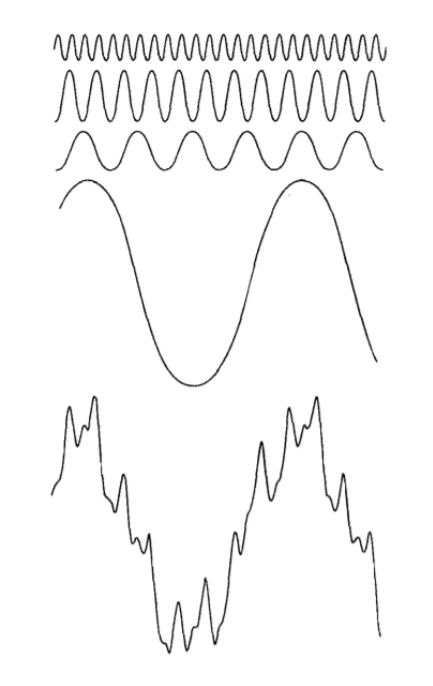
\includegraphics[scale=0.4]{Figures/fourier_example.png}
    \par \textbf {Hình 1.2} Ví dụ về chuỗi Fourier, hàm sóng cuối cùng là tổ hợp tuyến tính của các hàm sóng phía trên. 
\end{center}
Chuỗi Fourier của hàm tuần hoàn $p(t)$ có chu kì $T$ là:
\begin{equation}
  p(t) = \sum\limits_{n =  - \infty }^{ + \infty } {{c_n}{e^{j\frac{{2\pi n}}{T}t}}}. \tag{1.2-1}  
\end{equation}
Ta có công thức Euler trong trường số phức:
\begin{equation}
{e^{j\theta }} = \cos \theta  + i\sin \theta. \tag{1.2-2}
\end{equation}
Như vậy viết lại (1.2-1) ta được:
$$p(t) = \sum\limits_{n =  - \infty }^{ + \infty } {{c_n}(\cos (\frac{{2\pi n}}{T}t) + j\sin (\frac{{2\pi n}}{T}t))}.$$
\\
Trong đó:
\par $w=2\pi f=\frac{2\pi}{T}$
\par $w$ là tần số góc,
\par $f$ là tần số,
\par $T$ là chu kì,
\par $j$ là biến phức.

\subsection{Biến đổi Fourier cho hàm liên tục}
\subsubsection{Hàm một biến số}
Biến đổi Fourier thực chất là dạng biến đổi tổng quát từ khái niệm chuỗi Fourier.
Biến đổi Fourier của một hàm số liên tục $p(t)$, kí hiệu là $\mathcal{F} \{p(t)\}$ có công thức như sau:
\begin{equation}
\mathcal{F} \{p(t)\} = 
F(w ) = \int\limits_{ - \infty }^{ + \infty } {p(t){e^{ - jwt}}dt}.\tag{1.2-3}
\end{equation}
Ngược lại, cho trước hàm $F(w)$, ta có thể tìm lại hàm $p(t)$ bằng cách sử dụng biến đổi Fourier ngược (Inverse Fourier Transform):
\begin{equation}
\mathcal{F} ^{-1}\{F(w)\} = p(t) = \frac{1}{2\pi}\int\limits_{ - \infty }^{ + \infty } {F(w){e^{jwt}}dw} .\tag{1.2-4}
\end{equation}
Chứng minh:
Áp dụng công thức (1.2-3) cho vế phải, ta được:
\begin{equation*}
	\begin{split}
    VP & = \frac{1}{2\pi}\int\limits_{ - \infty }^{ + \infty } {F(w){e^{jwt}}dw} = \frac{1}{{2\pi }}\int\limits_{ - \infty }^{ + \infty } {(\int\limits_{ - \infty }^{ + \infty } {p(s){e^{ - jws}}ds){e^{jwt}}dw } } \\
    & = \frac{1}{{2\pi }}\int\limits_{ - \infty }^{ + \infty } {ds\,p(s)\,\int\limits_{ - \infty }^{ + \infty } {dw\,{e^{jw(t - s)}}} } \\
    & =\frac{1}{{2\pi }}\mathop {\lim }\limits_{N \to  + \infty } \int\limits_{ - \infty }^{ + \infty } {ds\,p(s)\,\frac{{{e^{j(t - s)N}} - {e^{ - j(t - s)N}}}}{{j(t - s)}}}.
	\end{split}
\end{equation*}

Áp dụng hệ quả công thức Euler (1.2-2):
$$VP=\frac{1}{{\pi }}\mathop {\lim }\limits_{N \to  + \infty } \int\limits_{ - \infty }^{ + \infty } {ds\,p(s)\,\frac{{\sin (N(t - s))}}{{t - s}}}
$$
Áp dụng shifting-property [3]:
\begin{equation*}
	\begin{split}
	VP &= \frac{1}{\pi }p(t)\mathop {\lim }\limits_{N \to  + \infty } \int\limits_{ - \infty }^{ + \infty } {ds} \frac{{\sin (N(t - s))}}{{t - s}} \\
	& = \frac{1}{\pi }p(t)\int\limits_{ - \infty }^{ + \infty } {dy} \frac{{\sin y}}{y} = p(t).
	\end{split}
\end{equation*}

Như vậy, ta được điều phải chứng minh.\\
\\
\textbf{Điều kiện áp dụng biến đổi Fourier}
\begin{itemize}
    \item $p(t)$ khả tích tuyệt đối
    $$\int\limits_{ - \infty }^{ + \infty } {|p(t)|dt < } \,\,\infty
.$$
    \item Trong một khoảng hữu hạn của $t$, $p(t)$ có hữu hạn cực đại và cực tiểu.
    \item Trong một khoảng hữu hạn của $t$, $p(t)$ có hữu hạn các điểm không liên tục và giá trị không liên tục là hữu hạn.
\end{itemize}

Ví dụ:
$$p(t) = \left\{ {\begin{array}{*{20}{c}}
{{e^{ - at}}\,\,\,\,(t > 0)}\\
{0\,\,\,\,(t < 0)}
\end{array}} \right.\,\,\,\,\,\,\,\,\,,\,a > 0.$$
Sử dụng định nghĩa (1.2-3), biến đổi Fourier của hàm số $p(t)$ trên là:
$$F(w) = \int\limits_{ - \infty }^{ + \infty } {p(t){e^{ - jwt}}dt = \int\limits_0^{ + \infty } {{e^{ - (a + jw)t}}dt = \frac{1}{{a + jw}}} } .$$
\subsubsection{Hàm hai biến số}
Với hàm hai biến số, ta có công thức biến đổi Fourier như sau:
\begin{equation}
\mathcal{F} \{p(x, y)\} = F(u,v) = \int\limits_{ - \infty }^{ + \infty } {\int\limits_{ - \infty }^{ + \infty } {p(x,y){e^{ - j({\rm{ux}} + vy)}}dx\,dy} }.\tag{1.2-5}
\end{equation}
Công thức biến đổi Fourier ngược
\begin{equation}
\mathcal{F}^{-1} \{F(u, v)\} = p(x,y) = \frac{1}{{4{\pi ^2}}}\int\limits_{ - \infty }^{ + \infty } {\int\limits_{ - \infty }^{ + \infty } {F(u,v){e^{j({\rm{ux}} + vy)}}dx\,dy} } .\tag{1.2-6}
\end{equation}
\subsection{Biến đổi Fourier cho hàm rời rạc}
\subsubsection{Hàm một biến số}
Với dãy $\{x_n\}$, $n=0, 1, 2,... N-1$ ta xây dựng DFT cho $x_n$ như sau 
\begin{equation}
\mathcal{F} \{x_n\} = {X_k} = \sum\limits_{n = 0}^{N-1} {{x_n}{e^{ - j\frac{{2\pi n}}{N}k}}} .\tag{1.2-7}
\end{equation}
Công thức IDFT
\begin{equation}
\mathcal{F}^{-1}\{X_k\} = {x_k} = \frac{1}{N}\sum\limits_{n = 0}^{N-1} {{X_n}{e^{j\frac{{2\pi n}}{N}k}}} .\tag{1.2-8}
\end{equation}
Chứng minh:
Từ định nghĩa DFT (1.2-7), ta có:
$$\frac{1}{N}\sum\limits_{n = 0}^{N-1} {{X_n}{e^{j\frac{{2\pi n}}{N}k}}} = \frac{1}{N}\sum\limits_{n = 0}^{N-1} {{
(\sum\limits_{m = 0}^{N-1} {{x_m}{e^{ - j\frac{{2\pi m}}{N}n}}})
}{e^{j\frac{{2\pi n}}{N}k}}} $$
$$=\frac{1}{N}\sum\limits_{m = 0}^{N-1} {{x_m}\sum\limits_{n = 0}^{N-1} {{e^{j\frac{{2\pi (k - m)}}{N}n}}} }
.$$
Nếu $k=m$ thì $\sum\limits_{n = 0}^{N-1} {{e^{j\frac{{2\pi (k - m)}}{N}n}}}=N.$\\
Nếu $k\neq m$ thì áp dụng công thức cấp số nhân, ta được:
$$S = \sum\limits_{n = 0}^{N-1} {{e^{j\frac{{2\pi (k - m)}}{N}n}}}
= \frac{{1 - {e^{j\frac{{2\pi (k - m)}}{N}N}}}}{{1 - {e^{j\frac{{2\pi (k - m)}}{N}}}}} = \frac{{1 - {e^{j2\pi (k-m)}}}}{{1 - {e^{j\frac{{2\pi (k - m)}}{N}}}}}.$$
Áp dụng công thức Euler (1.2-2):
$${e^{j2\pi (k - m)}} = \cos (2\pi (k - m)) + i\sin (2\pi (k - m)) = 1 $$
và
$${e^{\frac{{^{j2\pi (k - m)}}}{N}}} \ne 1 .$$
Do đó $S=0$ khi $k\neq m$, như vậy ta có điều phải chứng minh
$$\frac{1}{N}\sum\limits_{n = 0}^{N-1} {{X_n}{e^{j\frac{{2\pi n}}{N}k}}}= \frac{1}{N}x_k N = x_k.$$
\subsubsection{Hàm hai biến số}
Tương tự, ta có khai triển DFT cho hàm hai biến số
\begin{equation}
\mathcal{F} \{p(x,y)\} = F(u,v) = \frac{1}{{MN}}\sum\limits_{x = 0}^{M - 1} {\sum\limits_{y = 0}^{N - 1} {p(x,y){e^{ - j2\pi (\frac{{ux}}{M} + \frac{{vy}}{N})}}} } .\tag{1.2-9}
\end{equation}
Khai triển IDFT
\begin{equation}
\mathcal{F}^{-1} \{F(u,v)\}
p(x,y) = \sum\limits_{x = 0}^{M - 1} {\sum\limits_{y = 0}^{N - 1} {F(u,v){e^{j2\pi (\frac{{ux}}{M} + \frac{{vy}}{N})}}} }.\tag{1.2-10}
\end{equation}
\subsection{Tính chất}
Ta có một số tính chất cơ bản của phép biến đổi Fourier như sau:
\begin{itemize}
\item \textbf{Tính tuyến tính}
\par Nếu $F_1(w)\leftrightarrow p_1(t)$ và $F_2(w)\leftrightarrow p_2(t)$ \par thì $a_1 F_1(w) + a_2 F_2(w) \leftrightarrow a_1 f_1(t) + a_2 f_2(t) $, $a_1$, $a_2$ là các hằng số.


\item \textbf{Tính đối xứng (đối ngẫu thời gian - tần số)}
\par $p(t)\leftrightarrow F(w) \rightarrow F(t) \leftrightarrow 2\pi p(-w).$

\item \textbf{Tính đồng dạng}
\par $p(at)\leftrightarrow \frac{1}{|a|}F(\frac{w}{a}).$

\item \textbf{Tính dịch chuyển trong miền thời gian}
\par $p(t-t_0)\leftrightarrow {e^{ - jw{t_0}}}F(w).$

\item \textbf{Tính dịch chuyển trong miền tần số}
\par $p(t){e^{jw{t_0}}} \leftrightarrow F(w-w_0).$
\end{itemize}

\subsection{Thuật toán FFT (Fast Fourier Transform)}
Để biến đổi ảnh từ miền không gian sang miền tần số bằng cách sử dụng chuyển đổi Fourier rời rạc hai chiều thông thường đòi hỏi chi phí tính toán lớn khi kích thước ảnh lớn là $O(MN)$, hay đơn giản là $O(N^2)$ với $M,N$ là kích thước ảnh. Thuật toán FFT thực hiện giảm thiểu chi phí tính toán xuống $O(Nlog_2 N)$.
\par Thuật toán FFT thông dụng nhất là thuật toán do J.W.Cooley và John Tukey [4] đề xuất, biến đổi Fourier cho các giá trị rời rạc bằng cách sử dụng đệ quy tính các giá trị ở vị trí chẵn và lẻ. 
\subsubsection{FFT một chiều} 
\begin{align}
	{X_k} & = \sum\limits_{m = 0}^{\frac{N}{2}-1} {{x_{2m}}{e^{ - \frac{{j2\pi (2m)}}{N}k}}}  + \sum\limits_{m = 0}^{\frac{N}{2}-1} {{x_{2m + 1}}{e^{ - \frac{{j2\pi (2m + 1)}}{N}k}}} \notag \\
	& = \sum\limits_{m = 0}^{\frac{N}{2}-1} {{x_{2m}}{e^{ - \frac{{j2\pi m}}{{N/2}}k}}}  + {e^{ - \frac{{2\pi j}}{N}k}}\sum\limits_{m = 0}^{\frac{N}{2}-1} {{x_{2m + 1}}{e^{ - \frac{{j2\pi m}}{N/2}k}}} \notag \\
	& = E_k + {e^{ - \frac{{2\pi j}}{N}k}}O_k \tag{1.2-11}
\end{align}

với $E_k$ là DFT phần chẵn và $O_k$ là DFT phần lẻ. \\
Do tính tuần hoàn có chu kì nên
$E_{k+\frac{N}{2}}=E_k$
và
$O_{k+\frac{N}{2}}=O_k.$ \\
Khi đó, ta viết lại phương trình (1.2-11) thành
\begin{equation}
{X_k} = \left\{ {\begin{array}{*{20}{c}}
{{E_k} + {e^{ - \frac{{2\pi j}}{N}k}}{O_k}\,\,\,\,\,\,\,\,\,\,\,\,\,\,\,\,\,\,\,\,\,\,\,\,\,\,\,,\,0 \le k < \frac{N}{2}}\\
{{E_{k - N/2}} + {e^{ - \frac{{2\pi j}}{N}k}}{O_{k - N/2}}\,\,\,\,\,\,\,\,\,\,,\,\frac{N}{2} \le k < N.}
\end{array}} \right. \tag{1.2-12}
\end{equation} \\
Mặt khác, ta có
$${e^{ - \frac{{2\pi j}}{N}(k + N/2)}} = {e^{ - \frac{{2\pi j}}{N}k - \pi j}} =  - {e^{ - \frac{{2\pi j}}{N}k}}.$$ \\
Như vậy, ta có thể giảm khối lượng tính toán xuống một nửa. Với $0\le K < \frac{N}{2}$, từ phương trình (1.12-12) ta thu được:
$${X_k} = {E_k} + {e^{ - \frac{{2\pi j}}{N}k}}{O_k}
$$
$${X_{k + N/2}} = {E_k} - {e^{ - \frac{{2\pi j}}{N}k}}{O_k}.
$$

\par Tính DFT cho tín hiệu rời rạc 1 chiều có $2^n$ phần tử cẩn tới $(2^n)^2$ phép nhân. Tuy nhiên áp dụng FFT chỉ cần $n^{2^n}$. Do đó, về cơ bản tốc độ tính toán nhanh hơn $\frac{2^n}{n}$ lần.\\
\begin{center}
\begin{tabular}{|l|l|l|l|}
\hline
\multicolumn{1}{|c|}{\multirow{2}{*}{Kích thước}} & \multicolumn{2}{c|}{Số phép nhân} & \multicolumn{1}{c|}{\multirow{2}{*}{Tỉ lệ}} \\ \cline{2-3}
\multicolumn{1}{|c|}{}                            & Định nghĩa         & FFT          & \multicolumn{1}{c|}{}                                          \\ \hline
4                                                 & 16                 & 8            & 2.0                                                            \\ \hline
8                                                 & 84                 & 24           & 2.7                                                            \\ \hline
16                                                & 256                & 64           & 4.0                                                            \\ \hline
32                                                & 1024               & 160          & 6.4                                                            \\ \hline
64                                                & 4096               & 384          & 10.7                                                           \\ \hline
128                                               & 16384              & 896          & 18.3                                                           \\ \hline
256                                               & 65536              & 2048         & 32.0                                                           \\ \hline
512                                               & 262144             & 4608         & 56.0                                                           \\ \hline
1024                                              & 1048576            & 10240        & 102.4                                                          \\ \hline
\end{tabular}
\\
\end{center}
\begin{center}
    \textbf{Bảng 1.1:} So sánh thực hiện DFT theo định nghĩa và sử dụng FFT.
\end{center}

\begin{algorithm}[H]
	\SetAlgoLined
	\textbf{Input: }chuỗi số x, số lượng N, giá trị s.\\
	\textbf{Output: }chuỗi X = [X[0], X[1], ... X[N-1]].\\
	\textbf{function } X[0]...X[N-1] $\leftarrow$ $dfft$(x, N, s):\\
	\hspace{10mm} if N == 1 then \\
	\hspace{20mm} X[0] $\leftarrow$ x[0]\\
	\hspace{10mm} else\\
	\hspace{20mm} \# DFT cho X[0], X[2*s], X[3*s]...\\
	\hspace{20mm} X[0]...X[N/2-1] $\leftarrow$ $dfft$(x, N/2, 2s)\\
	\hspace{20mm} \# DFT cho X[s], X[3*s], X[5*s]...\\
	\hspace{20mm} X[N/2]...X[N-1] $\leftarrow$ $dfft$(x+s, N/2, 2s)\\
	\hspace{20mm} \# Kết hợp 2 nửa DFT thành 1 DFT\\
	\hspace{20mm} for k = 0 to N/2-1\\
	\hspace{30mm} t $\leftarrow$ X[k]\\
	\hspace{30mm} X[k] $\leftarrow$ t + exp(-2*PI*j*k/N)*X[k+N/2]\\
	\hspace{30mm} X[k+N/2] $\leftarrow$ t - exp(-2*PI*j*k/N)*X[k+N/2]\\
	\hspace{20mm} endfor\\
	\hspace{10mm} endif\\
	\caption{Thuật toán FFT - Fast Fourier Transform}
\end{algorithm}

\subsubsection{FFT hai chiều}
\par Ta có biến đổi dựa trên phương trình (1.2-9):
\begin{align*}
	\mathcal{F} \{p(x,y)\} & = F(u,v) = \frac{1}{{MN}}\sum\limits_{x = 0}^{M - 1} {\sum\limits_{y = 0}^{N - 1} {p(x,y){e^{ - j2\pi (\frac{{ux}}{M} + \frac{{vy}}{N})}}} } \\
	& = \frac{1}{M}\sum\limits_{x = 0}^{M - 1} {{e^{ - j2\pi \frac{{{\rm{ux}}}}{M}}}} \left[ {\frac{1}{N}\sum\limits_{y = 0}^{N - 1} {p(x,y){e^{ - j2\pi \frac{{vy}}{N}}}} } \right].
\end{align*}
Như vậy, biến đổi FFT hai chiều có thể được thực hiện bằng cách áp dụng biến đổi FFT một chiều trên từng hàng, sau đó biến đổi FFT trên từng cột.
\subsection{Định lý tích chập}
Cho hai hàm số liên tục $g(t)$ và $h(t)$, tích chập $*$ của hai hàm số này là
$$g(t)*h(t) = \int\limits_{ - \infty }^{ + \infty } {g(\tau )h(t - \tau )} d\tau .
$$
Áp dụng biến đổi Fourier sau khi sử dụng tích chập
$$\mathcal{F} \{g(t) * h(t)\} = \int\limits_{- \infty }^{ + \infty } \left[ \int\limits_{- \infty}^{+ \infty } g(\tau )h(t - \tau )d\tau  \right] e^{-jwt} dt.$$
Bằng phép đổi thứ tự lấy tích phân, ta được:
$$\mathcal{F} \{g(t) * h(t)\} = \int\limits_{ - \infty }^{ + \infty } {g(\tau ) \left[ \int\limits_{ - \infty }^{ + \infty } {h(t - \tau ) e^{-jwt}} dt \right] d\tau }.$$
Thực hiện phép đổi biến số $x=t-\tau$, ta được:
\begin{align*}
	\mathcal{F} \{g(t) * h(t)\} & =  \int\limits_{ - \infty }^{ + \infty } {g(\tau ) \left[ \int\limits_{ - \infty }^{ + \infty } {h(x) e^{ - j w(x + \tau ) } dx} \right] d\tau } \\
	& = \int\limits_{ - \infty }^{ + \infty } g(\tau ) \left[ \int\limits_{ - \infty }^{ + \infty } h(x)e^{ - jwx} dx \right] {{e}^{ - j w \tau }} d \tau \\
	& = H(w) \int\limits_{ - \infty }^{ + \infty } g(\tau ) { e^{ - jw \tau }}d\tau \\
	& = H(w)G(w),
\end{align*}

với $H(w)$, $G(w)$ là biến đổi Fourier của $h(t)$, $g(t)$.\\
Như vậy ta có:
$$\mathcal{F} \{g(t) * h(t)\} = H(w)G(w).$$
Định lý tích chập cho ta biết mối quan hệ giữa miền không gian và miền tần số, cụ thể, thông qua tích chập, một ảnh trong miền không gian có thể chuyển qua miền tần số và ngược lại. Phép tích chập được sử dụng trong miền không gian có thể được đơn giản hóa bằng phép nhân trong miền tần số thông qua biến đổi Fourier, thông qua đó tối thiểu hóa được chi phí tính toán. 
\section{Biến đổi Fourier trong xử lý ảnh số}
Biến đổi Fourier được sử dụng trong xử lý ảnh số chủ yếu là biến đổi Fourier rời rạc, vì mỗi bức ảnh được mã hóa dưới dạng ma trận hai chiều (đối với ảnh xám) và ba chiều (đối với ảnh màu thông thường như RGB, LAB, HSV,...). Đối với ảnh xám, mỗi điểm ảnh có giá trị từ 0 đến 255 biểu diễn cường độ ảnh. Do đó cường độ của điểm ảnh là một hàm số theo tọa độ trục tung và trục hoành tương ứng với vị trí của điểm ảnh đó.
\par Trong miền không gian, ta xử lý trực tiếp trên từng điểm ảnh, còn trong miền tần số, ta xử lý dựa trên tốc độ thay đổi giá trị trên miền không gian. Miền tần số có thể tạo ra mối quan hệ chu kỳ rõ ràng, giúp cho một số toán tử xử lý ảnh trở nên hiệu quả hơn, hoặc được đơn giản hóa chi phí tính toán. Do vậy, phép biến đổi Fourier đã được ứng dụng như một công cụ hữu hiệu để giải quyết các bài toán liên quan đến xử lý ảnh số.
\par Đối với bài toán phân đoạn ảnh (image segmentation), Paquet (1993)[17] giới thiệu cách tiếp cận mới để phân chia các mặt phẳng và tứ giác của hình ảnh 3D thông qua việc sử dụng biến đổi Fourier lên ảnh pha. Li và Wilson (1995)[12] đã xây dựng biến đổi Fourier đa phân giải (Multi Resolution Fourier Transform) để tiếp cận phân đoạn hình ảnh dựa trên phân tích thông tin địa phương trong miền không gian. Wu (1996)[23] đã trình bày thuật toán phân đoạn hình ảnh tế bào lặp bằng cách sử dụng các vectơ cường độ biến đổi Fourier thời gian ngắn như một đặc trưng của các lớp. Escofet (2001)[7] áp dụng biến đổi Fourier để phân đoạn hình ảnh và nhận dạng mẫu. Jianghong Li (2009)[13] sử dụng biến đổi Fourier trong việc phân đoạn các họa tiết động, nhằm xử lý chuỗi các hình ảnh thay đổi liên tiếp theo thời gian và không gian. 
\par Đối với bài toán phân loại hình ảnh (image classification), Grandlund (1972)[8] lần đầu tiên sử dụng biến đổi Fourier như một bước tiền xử lý trong việc nhận dạng ảnh kí tự viết tay. Robert (1980)[19] đã giới thiệu kĩ thuật phân loại hình ảnh vệ tinh tự động mà trong đó biến đổi Fourier rời rạc (DFT) được thiết kế để phát hiện và xác định tính năng của các đám mây từ mẫu hình ảnh chụp thường và hồng ngoại. Levchenko (1992)[11] đã thiết kết mô hình mạng nơron để phân loại hình ảnh đã được biến đổi Fourier. Harte và Hanka (1997)[9] đã xây dựng thuật toán cho vấn đề phân loại hình ảnh với kích thước lớn sử dụng biến đổi Fourier nhanh (FFT). Thông qua đó giải quyết được vấn đề về khối lượng tính toán đối với dữ liệu nhiều chiều. Tang và Stewart (2000)[21] sử dụng biến đổi Fourier để phân loại hình ảnh quang học. Hiệu suất phân loại của biến đổi Fourier được so sánh với biến đổi wavelet. Li-Wei Yang (2012)[14] sử dụng FFT trong nhận diện lá cây. Sokołowski (2014)[1] sử dụng trong phân loại ảnh nhận diện khối u ác tính. Popa (2018)[5] sử dụng FFT kết hợp với Complex-value Convolution Neural Network (CVCNNs) trong phân loại hình ảnh để tận dụng cả phần thực và phần ảo sau biến đổi, chỉ ra sự cải thiện độ chính xác so với chỉ sử dụng CNN trên trường số thực.
\par Biến đổi Fourier còn được sử dụng trong việc tái kết cấu ảnh (image reconstruction) như Matt Pharr (2004)[10] sử dụng thuật toán FFT trong việc tái kết cấu ảnh y tế, hay Rowe (2007)[6] sử dụng biến đổi Fourier để tái tạo tín hiệu và nhiễu của dữ liệu fMRI sử dụng thông tin của các ảnh pha sau biến đổi Fourier.
\par Trong những năm gần đây, với sự phát triển nhanh chóng của các ngành 4.0 như khoa học dữ liệu, trí tuệ nhân tạo, dữ liệu lớn,... biến đổi Fourier sử dụng trong xử lý ảnh số trong các thao tác tiền xử lý như lọc nhiễu, giảm mờ, sinh dữ liệu, trích chọn đặc trưng thô,... nhằm phục vụ cho mô hình mạng nơron học sâu. Trong khuôn khổ nội dung tiếp theo của đồ án sẽ trình bày về một số phương pháp tiền xử lý dữ liệu hình ảnh thông dụng và phương pháp trích chọn đặc trưng dựa trên biến đổi Fourier để xử lý bài toán nhận dạng mẫu.
%\begin{itemize}
%    \item Nén ảnh (ví dụ như chuẩn ảnh JPEG)
%item Lọc ảnh
%    \item Giảm mờ, nhiễu ảnh
%\end{itemize}
%Ngoài ra biến đổi Fourier còn được sử dụng nhưng một phương pháp %trích chọn đặc trưng sử dụng trong các mô hình nhận dạng như nhận %dạng khuôn mặt, nhận dạng kí tự viết tay




% ---------------------------------------------------------------------------- %
% Chapter 2 - 
\chapter{Một số ứng dụng của biến đổi Fourier}\label{CH2}
\section{Lọc ảnh trong miền tần số}
Đối với mỗi bức ảnh, những ảnh có tần số thấp là ảnh có sự thay đổi mức xám ít, ví dụ như ảnh một bức tường, mặt biển,... hay ảnh có tần số cao khi thay đổi mức xám đột ngột như biên của vật thể. Vì vậy, trong nhiều trường hợp ta cần có bộ lọc $H(u,v)$ thể làm giảm đi tần số cao trong khi đi qua các tần số thấp (gọi là lọc thông thấp) làm cho ảnh mờ đi, hay bộ lọc có tính chất ngược với lọc thông thấp (gọi là lọc thông cao) giúp tăng cường chi tiết hình dạng vật thể, đồng thời tăng độ tương phản ảnh. Đồ án sẽ đề cập đến các bộ lọc và ứng dụng của chúng.
%\begin{itemize}
%    \item Lọc thông thấp Ideal (Ideal low pass filter)
%    \item Lọc thông thấp Gaussian (Gaussian low pass filter)
%    \item Lọc thông thấp Butterworth (Butterworth low pass filter)
%    \item Lọc thông cao Ideal (Ideal high pass filter)
%    \item Lọc thông cao Gaussian (Gaussian high pass filter)
%    \item Lọc thông cao Butterworth (Butterworth high pass filter)
%\end{itemize}
\subsection{Lọc thông thấp}
\par Lọc thông thấp Ideal:
$$H(u,v) = \left\{ {\begin{array}{*{20}{c}}
{1\,\,\,\,if\,D(u,v)\, \le \,{D_0}}\\
{0\,\,\,\,if\,D(u,v)\, > \,{D_0}.}
\end{array}} \right.$$
Lọc thông thấp Gaussian:
%$$G(x,y) = \frac{1}{{2\pi {\sigma ^2}}}{e^{ - {\textstyle{{{x^2} + {y^2}} \over %{2{\sigma ^2}}}}}}$$

%Như vậy, ta có công thức của bộ lọc Gaussian:
$$H(u,v) = \frac{1}{{2\pi {\sigma ^2}}}{e^{ - {\textstyle{{{D^2}(u,v)} \over {2{\sigma ^2}}}}}}.$$
Lọc thông thấp Butterworth
$$H(u,v) = \frac{1}{{1 + {{\left[ {\frac{{D(u,v)}}{{{D_0}}}} \right]}^{2n}}}}$$
\\
trong đó $D_0$ là hằng số dương và $D(u,v)$ là khoảng cách giữa điểm $(u,v)$ trong miền tần số và tâm của hình chữ nhật tần số, tức là:
$$D(u,v) = \sqrt {{{(u - \frac{{\rm{W}}}{2})}^2} + {{(v - \frac{{\rm{H}}}{2})}^2}} $$
hoặc công thức đã được chuẩn hóa:
$$D(u,v) = \sqrt {{{(0.5 - \frac{u}{{\rm{W}}})}^2} + {{(0.5 - \frac{v}{H})}^2}} $$
với W, H lần lượt là chiều dài và chiều rộng của bức ảnh, $\sigma$ là độ lệch chuẩn trong hàm Gaussian và $n$ là cấp của bộ lọc Butterworth.
\begin{center}
    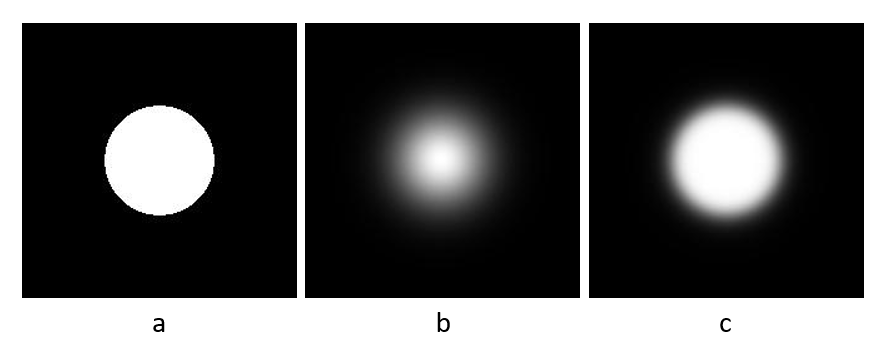
\includegraphics[scale=0.55]{Figures/fig6.png}
    \par \textbf {Hình 2.1} Bộ lọc thông thấp (a: Ideal, b: Gaussian, c: Butterworth).
\end{center}
\par Ảnh đầu vào sau khi thông qua biến đổi Fourier sẽ được nhân pixel-by-pixel với bộ lọc, kết quả thu được thông qua biến đổi Fourier ngược sẽ là ảnh đã được lọc.
\begin{center}
    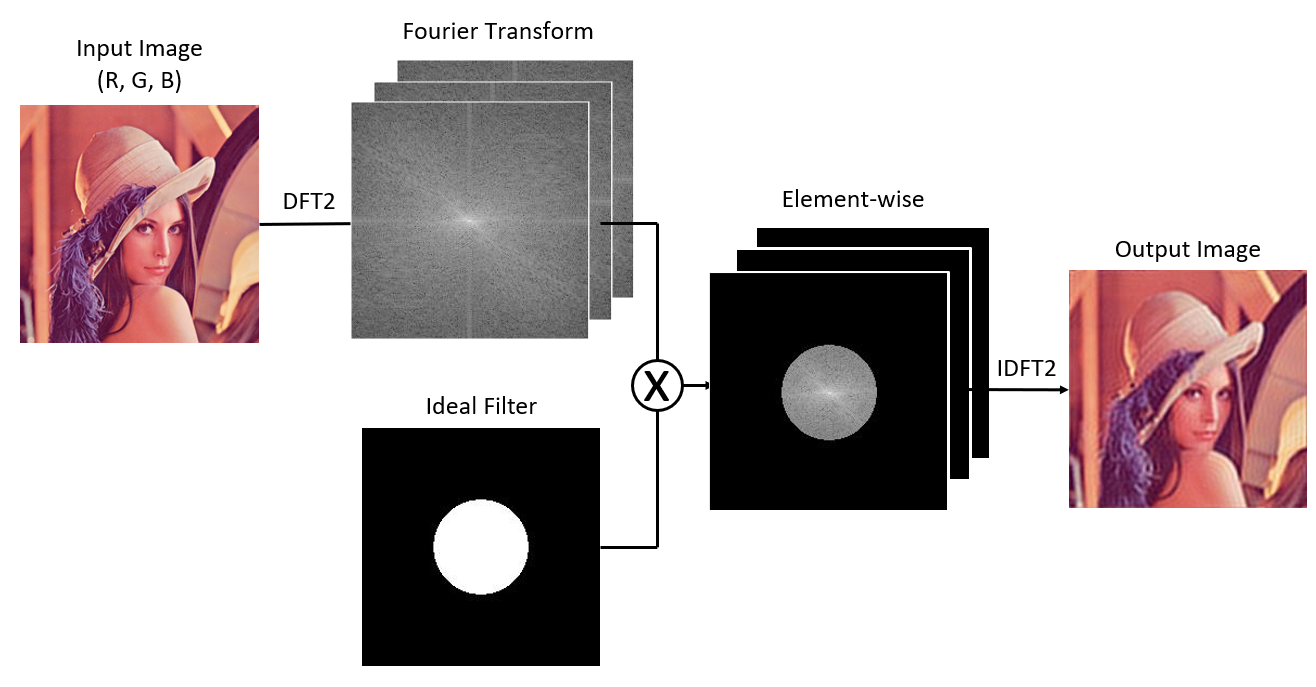
\includegraphics[scale=0.45]{Figures/fig1.png}
    \par \textbf {Hình 2.2} Lọc ảnh màu trong miền tần số bằng bộ lọc thông thấp Ideal.
\end{center}

Ảnh màu được cấu tạo bằng nhiều kênh màu khác nhau, thông dụng nhất là ảnh màu RGB với tương ứng 3 kênh màu Red-Green-Blur. Trong trường hợp muốn áp dụng bộ lọc cho ảnh màu RGB, ta sẽ áp dụng bộ lọc với từng kênh màu, coi mỗi kênh màu là một bức ảnh xám và ảnh thu được sẽ là kết hợp từ các kênh màu đã được lọc (hình 2.2).
\par Mã nguồn cho lọc thông thấp Ideal như sau:

\begin{lstlisting}[language=Matlab]
function filted_img = filterIdealLowPass(img,D0)
    % FFT input image
    fft_img = fftshift(fft2(double(img)));
    % Create low pass Ideal filter
    [H,W,c] = size(img);
    ctx = (W-1)/2;
    cty = (H-1)/2;
    [x, y] = meshgrid(1:W, 1:H);
    mg = sqrt((x - ctx ).^2 + (y - cty).^2);
    filter = double(mg <= D0);
    % Element-wise multiply each channel with the filter
    im = zeros(size(img));
    for z = 1:c
        im(:,:,z) = fft_img(:,:,z) .* filter;
    end 
    % IFFT to get ouput image
    filted_img = ifft2(ifftshift(im));
end
\end{lstlisting}
Bằng việc thay cách tạo bộ lọc, ta có mã nguồn tương ứng cho lọc thông thấp Gaussian và Butterworth.

\begin{lstlisting}[language = Matlab]
function filted_img = filterGaussianLowPass(img,fc)
    % FFT input image
    fft_img = fftshift(fft2(double(img)));
    % Create low pass Gaussian filter
    [H,W,c] = size(img);
    ctx = (W-1)/2;
    cty = (H-1)/2;
    a = 1/(2*pi*sig*sig);
    b = 2*sig*sig;
    [x, y] = meshgrid(1:W, 1:H);
    D2 = (x - ctx ).^2 + (y - cty).^2;
    filter = a*exp(-D2/b);
    filter = filter/max(filter(:))
    % Element-wise multiply each channel with the filter
    im = zeros(size(img));
    for z = 1:c
        im(:,:,z) = fft_img(:,:,z) .* filter;
    end 
    % IFFT to get ouput image
    filted_img = ifft2(ifftshift(im));
end
function filted_img = filterButterworthLowPass(img, D0, n)
    % FFT input image
    fft_img = fftshift(fft2(double(img)));
    % Create low pass Butterworth filter
    [H,W,c] = size(img);
    ctx = (W-1)/2;
    cty = (H-1)/2;
    [x, y] = meshgrid(1:W, 1:H);
    D2 = (x - ctx ).^2 + (y - cty).^2;
    filter = 1./(1+ (D2/D0/D0).^n);
    filter = filter/max(filter(:))
    % Element-wise multiply each channel with the filter
    im = zeros(size(img));
    for z = 1:c
        im(:,:,z) = fft_img(:,:,z) .* filter;
    end 
    % IFFT to get ouput image
    filted_img = ifft2(ifftshift(im));
end
\end{lstlisting}
\par Sau quá trình lọc thông thấp (hình 2.3), ảnh đầu vào sẽ bị giảm các tần số cao, tức là bị làm mờ, độ nét các đường biên giữa vật thể với nền đã bị giảm xuống. Thông qua biểu đồ tần số của bộ lọc Gaussian (hình 2.4), ta có thể thấy sau khi qua bộ lọc biểu đồ trông mượt hơn so với ban đầu. Các tần số của ảnh đã được kéo giãn ra, điều đó có nghĩa là nhiều tần số cao đã được kéo xuống. Tùy vào tính chất của từng bộ lọc mà dẫn đến hiện tượng xuất hiện các đường biên mờ quanh đường biên của vật thể trong ảnh trong bộ lọc Ideal, hay hiện tượng mờ toàn cục của bộ lọc Gaussian. 
\begin{center}
    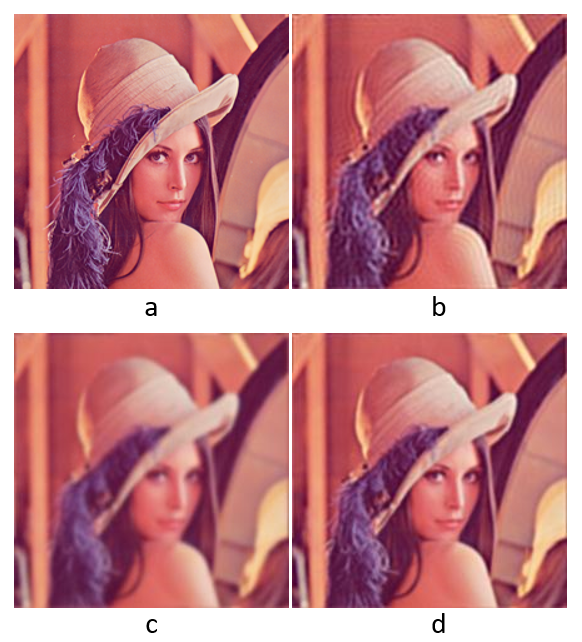
\includegraphics[scale=0.7]{Figures/fig8.png}
    \par \textbf {Hình 2.3} Kết quả sử dụng bộ lọc thông thấp\\ (a: ảnh gốc, b: Ideal, c: Gaussian, d: Butterworth).
\end{center}
\begin{center}
    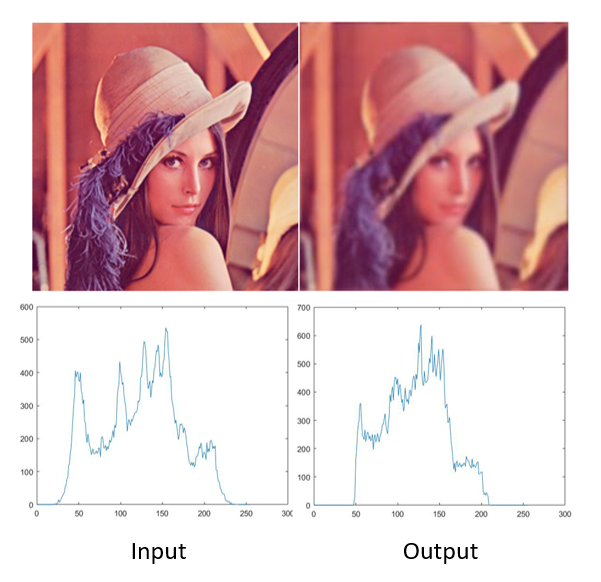
\includegraphics[scale=0.9]{Figures/fig7a.png}
    \par \textbf {Hình 2.4} Lọc thông thấp Gaussian.
\end{center}
\par Phép lọc thông thấp (lọc mờ ảnh) được ứng dụng trong nhận dạng ký tự quang học (OCR), công nghiệp in ấn, xử lý ảnh trên vệ tinh, tăng cường ảnh...

\subsection{Lọc thông cao}
Ngược lại với các bộ lọc thông thấp sẽ là các bộ lọc thông cao. Công thức cơ bản của các bộ lọc thông cao đó là:
$$Hi(u, v) = 1.0 - Lo(u, v)$$
trong đó $Lo(u,v)$ là bộ lọc thông thấp tương ứng mà giá trị mỗi điểm ảnh đã được chuẩn hóa trong đoạn $[0,1]$. Do vậy, ta thu được các bộ lọc như sau:
\begin{center}
    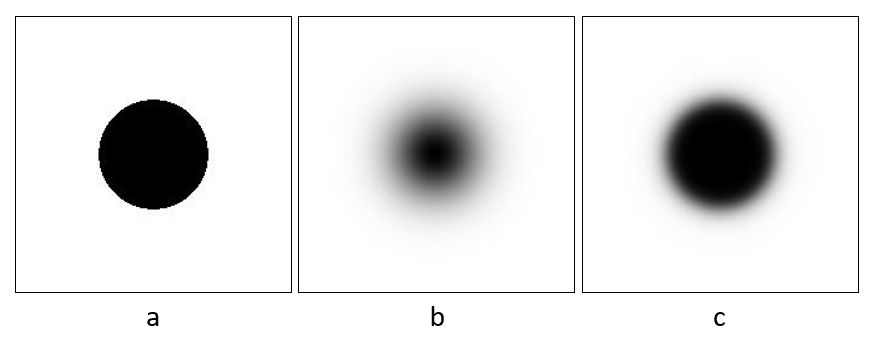
\includegraphics[scale=0.55]{Figures/fig9.png}
    \par \textbf {Hình 2.5} Bộ lọc thông cao (a: Ideal, b: Gaussian, c: Butterworth).
\end{center}
Tương tự như khi thực hiện lọc thông thấp, ta có mã nguồn cho thuật toán lọc thông cao:

\begin{lstlisting}[language=Octave]
function filted_img = filterIdealHighPass(img,D0)
    % FFT input image
    fft_img = fftshift(fft2(double(img)));
    % Create high pass Ideal filter
    [H,W,c] = size(img);
    ctx = (W-1)/2;
    cty = (H-1)/2;
    [x, y] = meshgrid(1:W, 1:H);
    mg = sqrt((x - ctx ).^2 + (y - cty).^2);
    filter = 1.0 - double(mg <= D0);
    % Element-wise multiply 
    im = zeros(size(img));
    for z = 1:c
        im(:,:,z) = fft_img(:,:,z) .* filter;
    end 
    % IFFT to get ouput image
    filted_img = ifft2(ifftshift(im));
end
function filted_img = filterGaussianHighPass(img,fc)
    % FFT input image
    fft_img = fftshift(fft2(double(img)));
    % Create high pass Gaussian filter
    [H,W,c] = size(img);
    ctx = (W-1)/2;
    cty = (H-1)/2;
    a = 1/(2*pi*sig*sig);
    b = 2*sig*sig;
    [x, y] = meshgrid(1:W, 1:H);
    D2 = (x - ctx ).^2 + (y - cty).^2;
    filter = a*exp(-D2/b);
    filter = 1.0 - filter/max(filter(:))
    % Element-wise multiply
    im = zeros(size(img));
    for z = 1:c
        im(:,:,z) = fft_img(:,:,z) .* filter;
    end 
    % IFFT to get ouput image
    filted_img = ifft2(ifftshift(im));
end
function filted_img = filterButterworthHighPass(img, D0, n)
    % FFT input image
    fft_img = fftshift(fft2(double(img)));
    % Create high pass Butterworth filter
    [H,W,c] = size(img);
    ctx = (W-1)/2;
    cty = (H-1)/2;
    [x, y] = meshgrid(-ctx:ctx, -cty:cty);
    D2 = (x/ctx).^2 + (y/cty).^2;
    filter = 1./(1+ (D2/D0/D0).^n);
    filter = 1.0 - filter/max(filter(:))
    % Element-wise multiply
    im = zeros(size(img));
    for z = 1:c
        im(:,:,z) = fft_img(:,:,z) .* filter;
    end 
    % IFFT to get ouput image
    filted_img = ifft2(ifftshift(im));
end
\end{lstlisting}
Để thuận tiện trong việc so sánh, kết quả của lọc thông cao sẽ được thực hiện trên ảnh xám. 
\begin{center}
    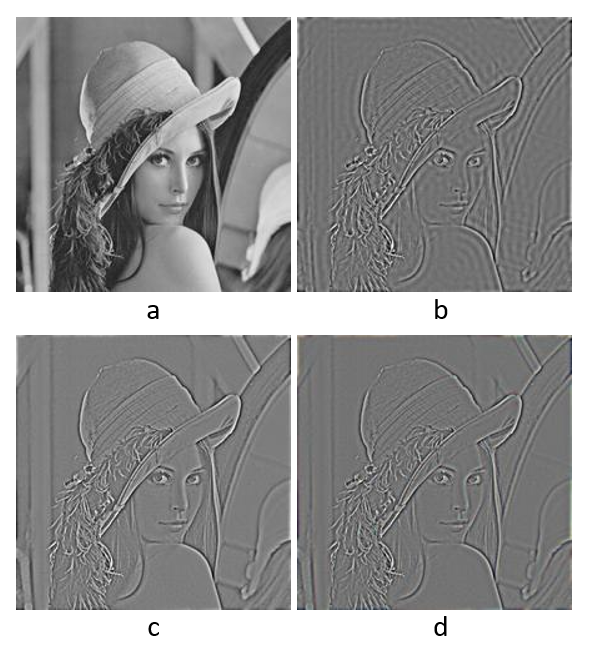
\includegraphics[scale=1.0]{Figures/fig10.png}
    \par \textbf {Hình 2.6} Kết quả sử dụng bộ lọc thông cao\\ (a: ảnh gốc, b: Ideal, c: Gaussian, d: Butterworth).
\end{center}
\par Lọc thông cao được ứng dụng trong việc hỗ trợ và trích xuất các đặc trưng đường, đặc trưng cạnh, làm nổi bật đường biên giữa vật thể và nền.

\section{Tăng cường ảnh}
\subsection{Lọc sắc ảnh dùng trong y tế}
Việc lọc sắc ảnh thường được thực hiện bằng cách cộng có trọng số ảnh gốc với ảnh đã thông qua lọc thông cao (kí hiệu là $HP$)[2]. Bằng cách làm này có thể làm nổi bật đặc trưng đường của ảnh, thông qua đó tăng cường chất lượng của các bộ lọc tiếp theo
$$Sharpen = Original + \lambda * HP$$
trong đó $\lambda$ thường được chọn trong khoảng $(0, 1)$. Mã nguồn của việc lọc sắc nét này như sau:

\begin{lstlisting}[language=Octave]
img = imread('input.jpg');
[H, W, c] = size(img);
img = rgb2gray(img);
weight = 0.5;
% sharpe = get_sharpen(img, 'IDEAL', 0.5);
% sharpe = get_sharpen(img, 'GAUSSIAN', 0.5);
sharpe = get_sharpen(img, 'BUTTERWORTH', 0.5);
function sharpe = get_sharpen(img, method, weight)
    high_pass = abs(get_high_pass(img, method));
    high_pass = mat2gray(high_pass) * 255.0;
    sharpe    = (double(img) + double(high_pass)*weight);
    sharpe    = uint8(sharpe);
end
function high_pass = get_high_pass(img, method)
    if string(method) == 'IDEAL'
        high_pass = IdealHighPass(img, 40);
    elseif string(method) == 'GAUSSIAN'
        high_pass = GaussHighPass(img, 20) ;
    else
        high_pass = ButterworthHighPass(img, 5, 30) ;
    end
end
\end{lstlisting}
Lấy ví dụ đối với bức ảnh chụp lát cắt não bộ và ảnh chụp X-Ray [2], ta thu được kết quả như sau:
\begin{center}
    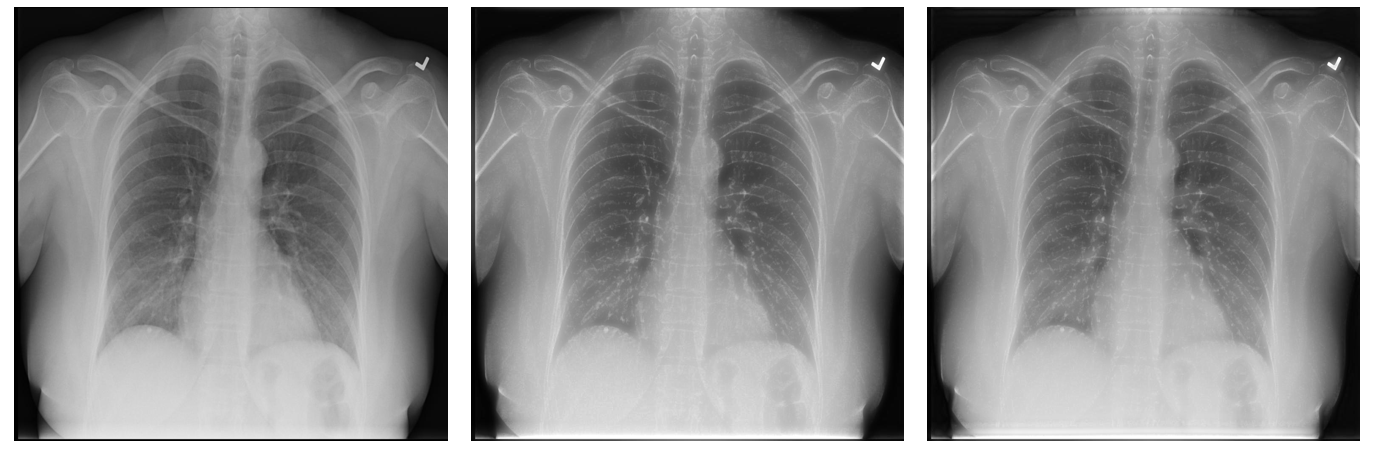
\includegraphics[scale=0.43]{Figures/fig14a.png}
    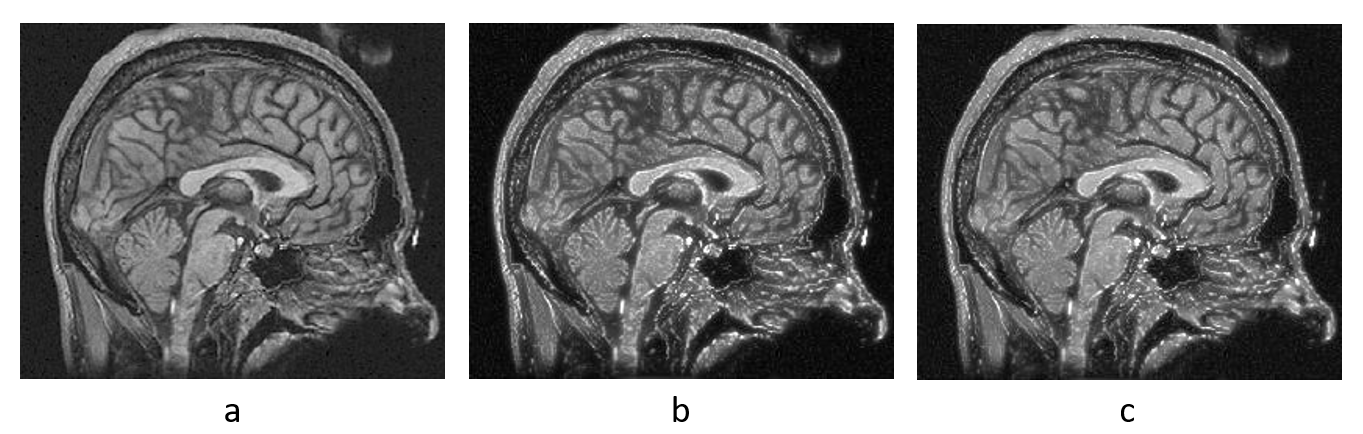
\includegraphics[scale=0.43]{Figures/fig14.png}
    \par \textbf {Hình 2.7} Lọc sắc nét ảnh X-Ray và MRI\\ (a: ảnh gốc, b: Gaussian, c: Butterworth).
\end{center}
Có thể thấy rằng sự tương phản trong ảnh được tăng lên, các đường biên trong ảnh đã được tăng cường và nổi bật hơn so với ảnh gốc. Ảnh chụp X-Ray thân trên của người có các đường biên ở xương sườn, xương cẳng tay, hệ thống mạch phía dưới phổi được kích sáng hơn, dễ dàng nhận diện các khu vực bị gãy, nứt. Ảnh MRI qua phép lọc nổi bật hơn và đồng thời cũng loại bỏ được phần nhiễu xung quanh.
\subsection{Lọc nhiễu ảnh trong nhận dạng vân tay}
Nhận dạng vân tay là một bài toán gặp nhiều khó khăn ở giai đoạn tiền xử lý. Ảnh vân tay thu được thường gặp những vết mờ, bẩn, nhiều nơi đường vân không rõ nét. 
\begin{center}
    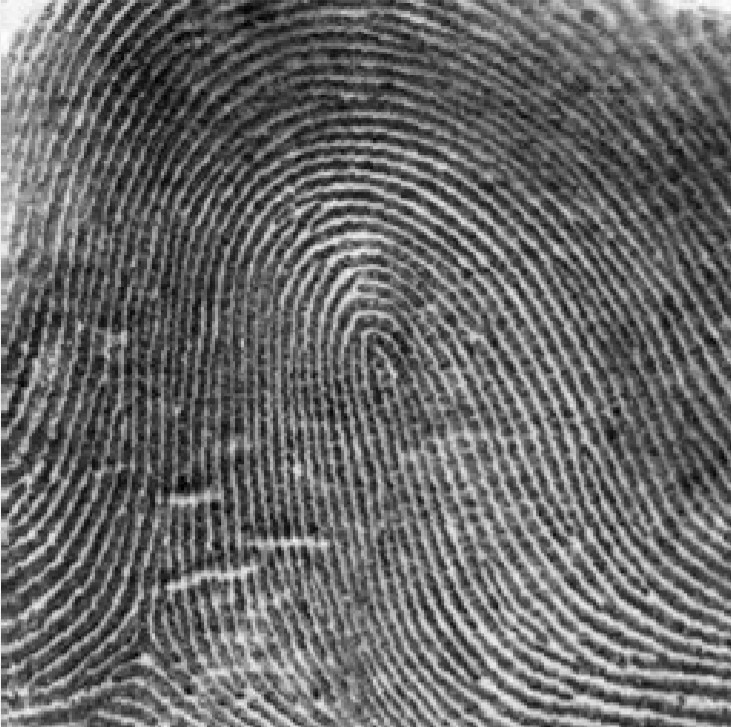
\includegraphics[scale=0.4]{Figures/anh_van_tay.jpg}
    \par \textbf {Hình 2.8} Ảnh mẫu vân tay.
\end{center}
Việc loại bỏ nhiễu có thể thực hiện đơn giản bằng phép lọc thông cao Butterworth, giúp giữ lại chỉ những đặc trưng đường vân quan trọng. Ta thu được kết quả sau khi sử dụng phép lọc thông cao Butterworth cấp 4:
\begin{center}
    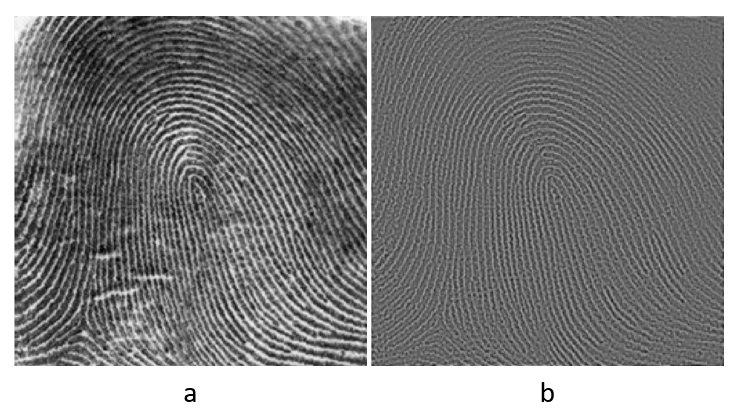
\includegraphics[scale=0.8]{Figures/fig13.png}
    \par \textbf {Hình 2.9} Khử nhiễu mẫu vân tay \\ (a: ảnh gốc, b: ảnh đã tăng cường).
\end{center}
Thông qua ảnh đã được lọc, đặc trưng có thể dễ dàng thu được phục vụ cho mục đích nhận dạng.
\subsection{Khử nhiễu ảnh trong công nghệ OCR}
Trong nền công nghiệp in ấn, đôi khi máy tính phải xử lý những bức ảnh chụp/scan chữ bị nhiễu, nhòe, mờ làm giảm chất lượng hình ảnh và gây khó khăn cho quá trình OCR (nhận diện kí tự quang học - Optical Characters Recognition). Để khắc phục điều này, giai đoạn tiền xử lý là tối quan trọng. Bên cạnh việc sử dụng việc áp dụng linh hoạt các phương pháp lọc, chẳng hạn lọc thông thấp giúp ảnh mượt (hình 2.11), thông qua phép biến đổi tích chập (convolution) và định lý tích chập được đề cập trong phần 1.2.5, các phép lọc ảnh sử dụng tích chập đã được sử dụng một cách phổ biến và linh hoạt, đặc biệt là các phép biến đổi hình học Morphology [16], mang lại nhiều tiện lợi và hiệu quả trong quá trình tiền xử lý hình ảnh.
\begin{center}
    
\includegraphics[scale=0.65]{Figures/fig15b.png}
    \par \textbf {Hình 2.10} Ảnh bị lỗi khi scan.
\end{center}
\begin{center}
    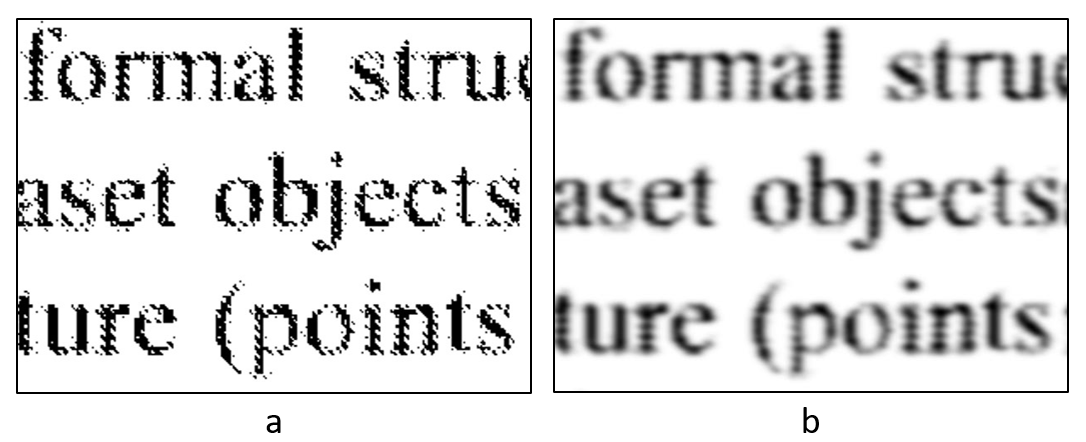
\includegraphics[scale=0.5]{Figures/fig11a.png}
    \par \textbf {Hình 2.11} Làm mượt ảnh trong bài toán OCR \\(a: ảnh nhiễu thu được từ máy in/scan, b: ảnh đã được làm mượt Gaussian).
\end{center}
Ta có thể tiến hành lọc ảnh bằng cách kết hợp nhiều phương pháp.

\begin{lstlisting}[language=Octave]
img = imread('input.png');
% Reverse image
img = 1.0 - double(img)/255.0;
% Create convolution-2D kernels
n = false(3);n(4) = 1;
s = false(3);s(6) = 1;
w = false(3);w(2) = 1;
e = false(3);e(8) = 1;
% Erode Morphology Mixture
fourNeighbourCount = imerode(img,n) + imerode(img,s) + imerode(img,w) + img;
img = fourNeighbourCount > 1;
% Smooth image using Low pass Gaussian
img = real(GaussLowPass(img, 30));
% Reverse again
imwrite(1.0-mat2gray(img), 'path-to-output-directory');
% Define Low-pass Filter Gaussian
function filted_img = GaussLowPass(img, sig)
    fft_img = fftshift(fft2(double(img)));
    [H,W,c] = size(img);
    ctx = (W-1)/2;
    cty = (H-1)/2;
    a = 1/(2*pi*sig*sig);
    b = 2*sig*sig;
    [x, y] = meshgrid(1:W, 1:H);
    D2 = (x - ctx ).^2 + (y - cty).^2;
    filter = a*exp(-D2/b);
    im = zeros(size(img));
    for z = 1:c
        im(:,:,z) = fft_img(:,:,z).*filter;
    end 
    filted_img = ifft2(ifftshift(im));
end
\end{lstlisting}
Bằng việc kết hợp giữa các toán tử biến đổi hình học Morphology (cụ thể trong trường hợp trên là phép lọc Erode [16]) và phép lọc thông thấp Gaussian, ta thu được kết quả tốt hơn so với việc chỉ sử dụng lọc thông thấp:
\begin{center}
    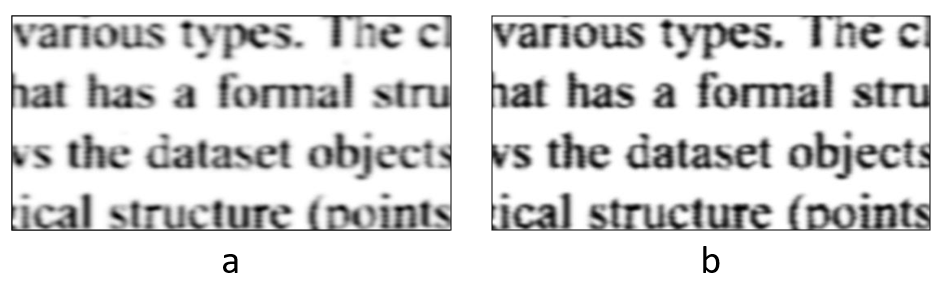
\includegraphics[scale=0.65]{Figures/fig15a.png}
    \par \textbf {Hình 2.12} Làm mượt ảnh trong bài toán OCR \\(a: ảnh được lọc thông thấp Gaussian, b: ảnh được lọc kết hợp).
\end{center}
Bên cạnh đó, phép lọc ngưỡng có thể được áp dụng sau phép lọc thông thấp trong trường hợp nền xung quanh chịu ảnh hưởng bởi nhiễu trong quá trình in ấn:
\begin{center}
    
\includegraphics[scale=0.50]{Figures/fig15c.png}
    \par \textbf {Hình 2.13} Làm mượt ảnh trong bài toán OCR \\(a: ảnh gốc, b: ảnh được lọc kết hợp với ngưỡng).
\end{center}
\subsection{Khử răng cưa}
Hiện tượng răng cưa (aliasing) xuất hiện khi ta thực hiện phục hồi ảnh từ ảnh đã thu nhỏ, hay phóng lớn ảnh từ ảnh kích thước nhỏ. Khử răng cưa (anti-aliasing) có thể được thực hiện đơn giản bằng phép làm mượt ảnh:
\begin{center}
    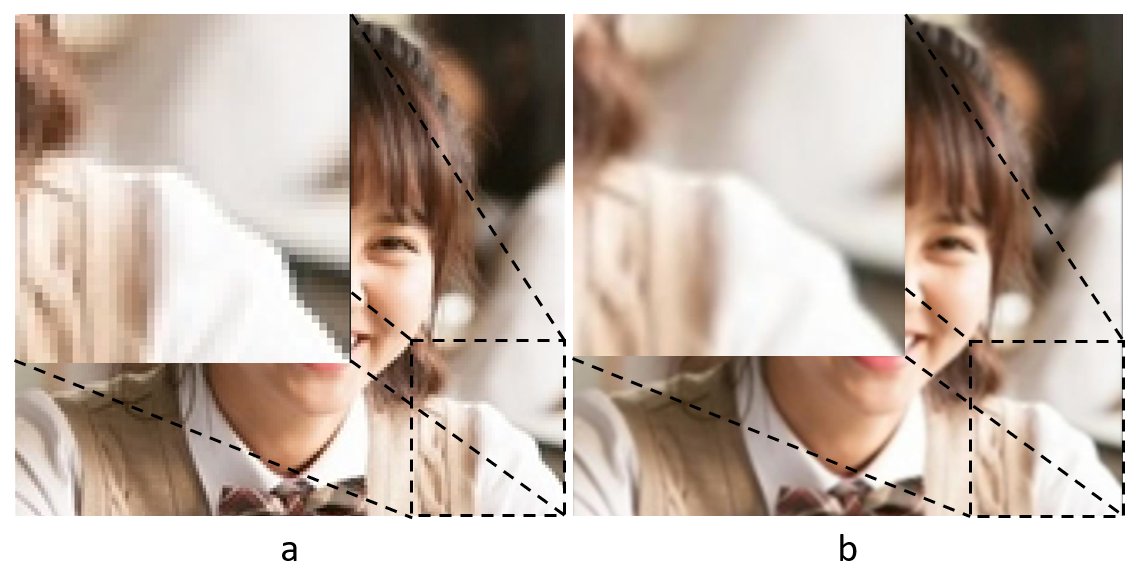
\includegraphics[scale=0.5]{Figures/fig16.png}
    \par \textbf {Hình 2.14} Khử răng cưa trong ảnh \\(a: ảnh bị răng cưa khi phóng lớn, b: ảnh được làm mượt bằng phép lọc Gaussian).
\end{center}
% ---------------------------------------------------------------------------- %
% Chapter 3 - 
\chapter{Ứng dụng DFT trong nén ảnh số}\label{CH3}
\par DFT và các biến đổi mang ý nghĩa tương đương khi biến đổi miền không gian sang miền tần số được ứng dụng trong việc nén ảnh số có và không mất mát thông tin mà trong đó, hiện nay ứng dụng rộng rãi nhất đó là kĩ thuật nén ảnh số JPEG. Các nghiên cứu về nén ảnh số xoay quanh vấn đề giảm thiểu dung lượng file ảnh gốc tuy nhiên vẫn giữ được chất lượng mà mắt con người vẫn có thể nhận biết rõ ràng. Đồ án sẽ xây dựng chương trình nén ảnh số dựa trên bài báo [15].
\section{Kĩ thuật đường ống}
Kĩ thuật đường ống của chương trình nén ảnh được thể hiện qua sơ đồ sau:
\begin{center}
    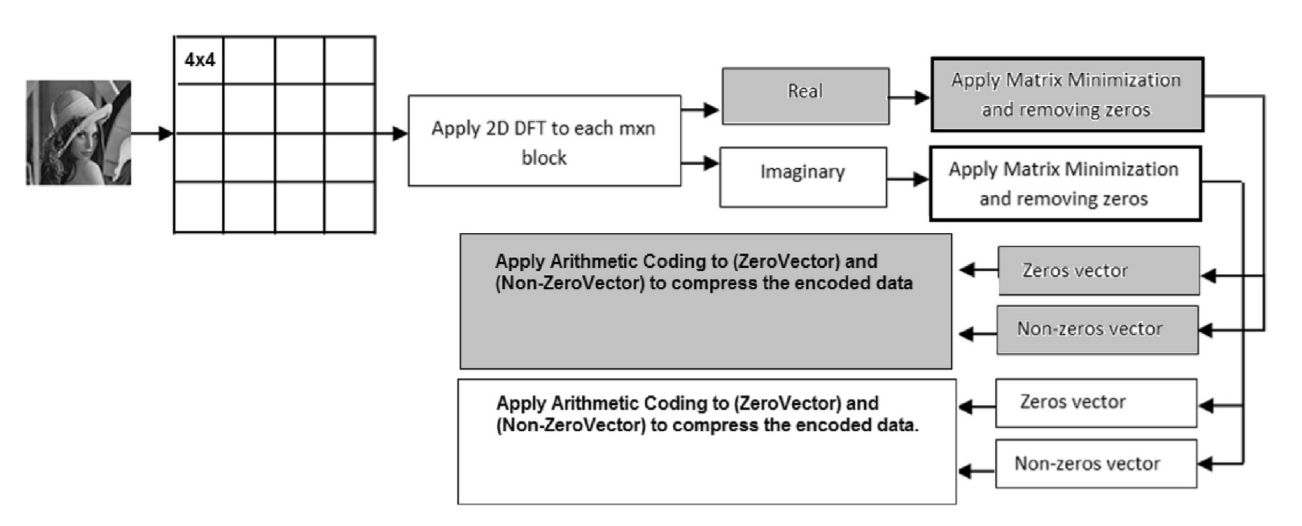
\includegraphics[scale=0.5]{Figures/fig17.png}
    \par \textbf {Hình 3.1} Phương án đề xuất [15].
\end{center}
\par Kĩ thuật nén ảnh được xây dựng dựa trên cơ sở ảnh đầu vào là ảnh xám, đối với ảnh màu có thể coi mỗi kênh màu là một ảnh xám và thực hiện nén trên từng kênh. Kết quả thu được sẽ được nối lại theo thứ tự. Mỗi bức ảnh xám ban đầu sẽ được thực hiện theo các bước như sau:
\subsection{Áp dụng DFT trên từng khối}
\par Việc thực hiện DFT trên từng khối, mặc định là khối có kích thước 4x4 sẽ đưa mỗi khối của ảnh gốc ban đầu từ miền không gian sang miền tần số. Giống như đã trình bày ở phần lọc ảnh, giá trị đầu tiên của mỗi khối là giá trị tần số thấp sẽ mang đặc trưng liên quan đến chi tiết, hình dạng của vật thể trong ảnh, sẽ được trích xuất ra một vector riêng và được bảo toàn nhằm giữ lại chất lượng hình ảnh một cách tốt nhất. Vector này được gọi là LFC (Low-Frequency-Components). Ma trận còn lại sau khi loại bỏ LFC được gọi là ma trận HFC (High-Frequency-Components) khi chỉ mang những giá trị tần số cao.

\begin{itemize}
    \item Nén: Thông qua ảnh ban đầu và biến đổi DFT trên từng khối trích xuất ma trận LFC và HFC.
    \item Giải nén: Từ vector LFC và HFC kết hợp với biến đổi IDFT trên từng khối thu được ảnh đã được giải nén. 
\end{itemize}

\begin{center}
    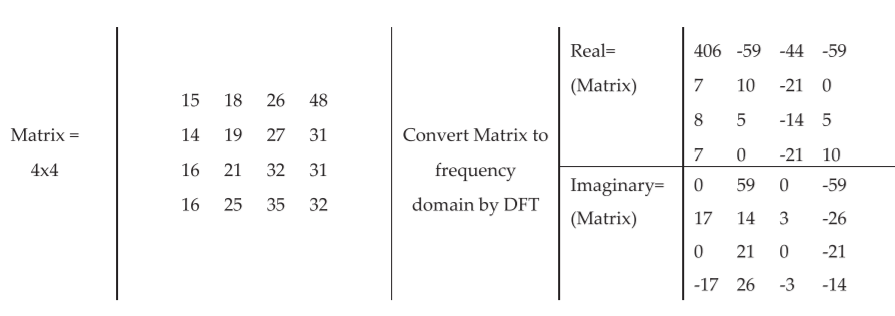
\includegraphics[scale=0.65]{Figures/fig18.png}
    \par \textbf {Hình 3.2} Biến đổi DFT trên từng khối [15].
\end{center}
\subsection{Lượng tử hóa}
\par Kĩ thuật lượng tử hóa (quantization) thường được sử dụng trong các phương pháp nén có mất mát dữ liệu. Các giá trị của vector hoặc ma trận sẽ được chia cho giá trị $q$ (ví dụ $q=20$) và được làm tròn đến số nguyên gần nhất. Quá trình giải nén dữ liệu sẽ được nhân với giá trị $q$ ban đầu.
\begin{center}
    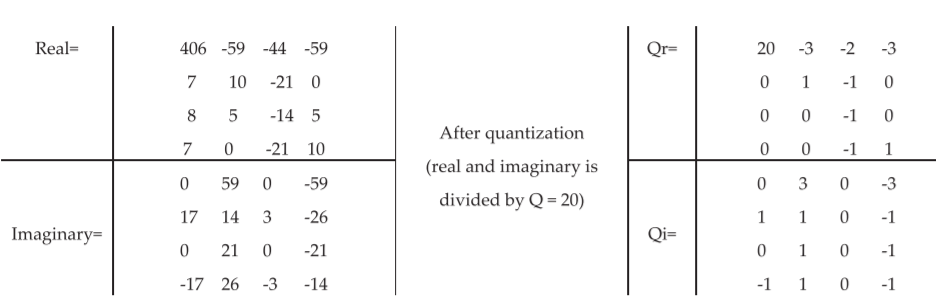
\includegraphics[scale=0.6]{Figures/fig19.png}
    \par \textbf {Hình 3.3} Quá trình lượng tử hóa [15].
\end{center}
\subsection{Áp dụng thuật toán Matrix Minimization [15]}
\par Thông qua việc trích xuất vector LFC và ma trận HFC và lượng tử hóa. Dễ thấy rằng kích thước LFC nhỏ hơn 16 lần (đối với khối có kích thước 4x4) so với kích thước HFC. Do vậy, ta cần phải nén ma trận HFC. Việc này được thực hiện bằng thuật toán Matrix Minimization [15].
\par Thuật toán sinh ngẫu nhiên 3 giá trị, thường nằm trong khoảng $(0, 1)$, thực hiện nhân với các khối không chồng lên nhau và cộng lấy giá trị cuối. Như vậy kích thước của vector đầu ra giảm 3 lần so với ban đầu. Khóa K và bảng giá trị Limited-data được lưu lại cho quá trình giải nén. Thuật toán giải nén được sử dụng là tìm kiếm tuần tự (Linear Sequential Search) tuy đơn giản nhưng chi phí tính toán cao.
\begin{itemize}
    \item Nén: thuật toán Matrix Minimization.
    \item Giải nén: thuật toán tìm kiếm tuần tự.
\end{itemize}

\begin{center}
    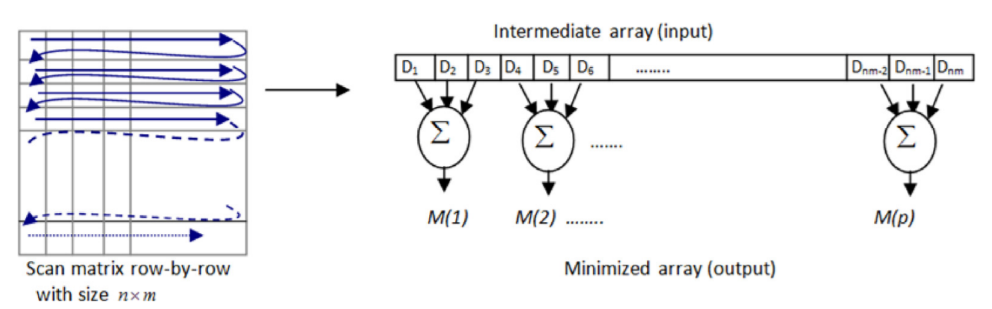
\includegraphics[scale=0.6]{Figures/fig21.png}
    \par \textbf {Hình 3.4} Thuật toán Matrix Minimization [15].
\end{center}
\begin{algorithm}[H]
%\SetAlgoLined
\textbf{Input: } Ma trận HFC.\\
\textbf{Output: } Ma trận HFC đã được tối thiểu hóa.\\
\textbf{function } HFC\_minimized $\leftarrow$ $MM$(HFC):\\
\hspace{10mm} \# Tạo 3 giá trị khóa ngẫu nhiên trong khoảng (0, 1)\\
\hspace{10mm} K = rand(1, 3)\\
\hspace{10mm} \# Duỗi thẳng ma trận HFC\\
\hspace{10mm} [height, width] $\leftarrow$ size(HFC)\\
\hspace{10mm} tmp $\leftarrow$ 1\\
\hspace{10mm} for i = 1 to height do\\
\hspace{20mm} for j = 1 to width do\\
\hspace{30mm} HFC\_flatted(tmp) $\leftarrow$ HFC(i, j)\\
\hspace{30mm} tmp $\leftarrow$ tmp + 1\\
\hspace{20mm} endfor\\
\hspace{10mm} endfor\\
\hspace{10mm} \# Lặp\\
\hspace{10mm} tmp $\leftarrow$ 1\\
\hspace{10mm} j $\leftarrow$ 1\\
\hspace{10mm} while (j < height * width) do\\
\hspace{20mm} sum $\leftarrow$ HFC\_flatted(j)*K(1) + HFC\_flatted(j+1)*K(2) + HFC\_flatted(j+2)*K(3) \\
\hspace{20mm} HFC\_minimized(tmp) $\leftarrow$ sum\\
\hspace{20mm} tmp $\leftarrow$ tmp + 1\\
\hspace{20mm} j $\leftarrow$ j + 3\\
\hspace{10mm} end\\
 \caption{Thuật toán Matrix Minimization Encoding}
\end{algorithm}


\subsection{Thuật toán Aritmetic Coding [15]}
\par Khái niệm entropy dùng để chỉ mức độ hỗn loạn của thông tin. Với một thông tin $x$ có thể nhận các giá trị $i$ với xác suất $p(i)$, entropy (kí hiệu là $S$) được định nghĩa theo công thức:
$$S =  - \sum\limits_i {p(i)\log (p(i))}.$$
\par Aritmetic Coding (AC) là thuật toán nén dữ liệu dựa trên lý thuyết thông tin, cho phép lưu trữ thông tin với số lượng bits tối thiểu. Claude Shannon chỉ ra rằng không thể nào lưu trữ thông tin với số bits nhỏ hơn entropy của thông tin này. AC cho phép tiến tới gần giới hạn entropy này với khoảng cách 2 bits.
\par Để đảm bảo hiệu quả cho thuật toán Aritmetic Coding, khi mà số lượng các giá trị 0 chiếm số lượng lớn trong dữ liệu, ta thực hiện việc tách vector HFC ban đầu thành 2 vector con định nghĩa phần giá trị khác 0 và giá trị bằng 0 (hình 3.5) và thực hiện mã hóa Aritmetic. 
\begin{center}
    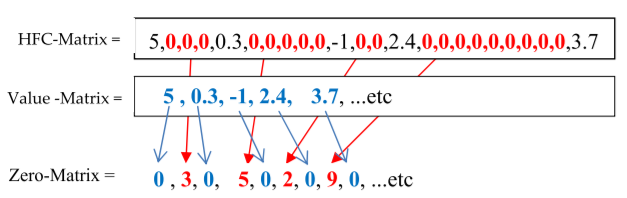
\includegraphics[scale=0.8]{Figures/fig22.png}
    \par \textbf {Hình 3.5} Tách vector HFC thành vector 0 và vector giá trị [15].
\end{center}
\section{Quá trình giải mã}
\par Quá trình giải nén được thực hiện tuần tự theo chiều ngược lại của quá trình nén, các bước như sau:
\begin{itemize}
    \item Áp dụng thuật toán giải nén Aritmetic Decoding.
    \item Kết hợp các vector 0 và vector giá trị để thu được vector HFC đã được tối thiểu và vector LFC.
    \item Thuật toán giải nén Matrix Minimization Decoding cho vector HFC tối thiểu để thu được vector HFC.
    \item Kết hợp vector HFC và vector LFC và thực hiện IDFT trên từng khối để thu được ảnh đã giải nén.
\end{itemize}
\par Quá trình giải nén được thể hiện qua sơ đồ sau:
\begin{center}
    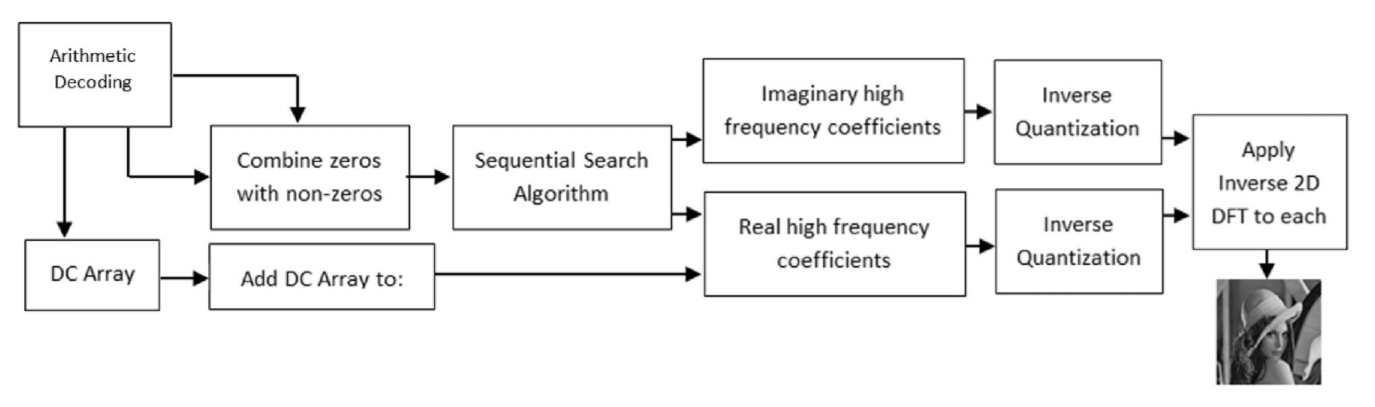
\includegraphics[scale=0.45]{Figures/fig23.png}
    \par \textbf {Hình 3.6} Sơ đồ giải nén ảnh [15].
\end{center}
\section{Kết quả}
\par Sự chênh lệch giữa ảnh gốc và ảnh đã nén và giải nén được đánh giá qua tiêu chuẩn RMSE:
$$RMSE(y, y') = \sqrt {\frac{{\sum\limits_{i = 1}^H {\sum\limits_{j = 1}^W {\sum\limits_{k = 1}^C {{{(y(i,j,k) - y'(i,j,k))}^2}} } } }}{{H.W.C}}}$$
với $y, y'$ lần lượt là ma trận ảnh gốc và ảnh sau khi giải nén, $H, W, C$ lần lượt là chiều rộng, chiều dài và số kênh màu của ảnh.
\par Thuật toán hoạt động khá tốt, nhưng gặp phải một số hạn chế nhất định như giá trị lượng tử hóa q được lựa chọn một cách heuristic [15] và những giá trị cao không thể hoạt động tốt trong tất cả các trường hợp. Ví dụ như giá trị lượng tử hóa cao vẫn giúp giữ lại chất lượng ảnh tốt cho dù định dạng TIF hay PNG và ảnh màu hay ảnh xám (hình 3.8, hình 3.9, hình 3.10), nhưng lại gây ra hiện tượng thay đổi rõ rệt chất lượng trong một số ảnh, đặc biệt là ảnh kích thước nhỏ (hình 3.7, hình 3.11). Và bên cạnh việc quá trình nén ảnh không tốn nhiều tài nguyên nhưng quá trình giải nén ảnh tốn khá nhiều tài nguyên và thời gian, chủ yếu ở thuật toán tìm kiếm tuần tự.
\par Kết quả của thuật toán nén ảnh được mô tả qua bảng 3.1.
\vspace{10mm}
\begin{center}
\begin{tabular}{|c|c|c|c|c|l|}
\hline
\multirow{2}{*}{Ảnh} & \multirow{2}{*}{\begin{tabular}[c]{@{}c@{}}Kích thước\\ 8-bits (kB)\end{tabular}} & \multirow{2}{*}{\begin{tabular}[c]{@{}c@{}}Kích thước \\ file (kB)\end{tabular}} & \multirow{2}{*}{q} & \multirow{2}{*}{\begin{tabular}[c]{@{}c@{}}Kích thước\\ nén (kB)\end{tabular}} & \multicolumn{1}{c|}{\multirow{2}{*}{RMSE}} \\
 &  &  &  &  & \multicolumn{1}{c|}{} \\ \hline
\multirow{3}{*}{\begin{tabular}[c]{@{}c@{}}lena.tif\\ (512x512)\end{tabular}} & \multirow{3}{*}{\begin{tabular}[c]{@{}c@{}}768\\ (color)\end{tabular}} & \multirow{3}{*}{768} & 10 & 614 & 1.9495 \\ \cline{4-6} 
 &  &  & 20 & 421 & 2.8530 \\ \cline{4-6} 
 &  &  & 40 & 253 & 24.2674 \\ \hline
\multirow{3}{*}{\begin{tabular}[c]{@{}c@{}}airplane.png\\ (512x512)\end{tabular}} & \multirow{3}{*}{\begin{tabular}[c]{@{}c@{}}768\\ (color)\end{tabular}} & \multirow{3}{*}{439} & 20 & 362 & 2.3843 \\ \cline{4-6} 
 &  &  & 40 & 213 & 5.5639 \\ \cline{4-6} 
 &  &  & 60 & 154 & 8.7267 \\ \hline
\multirow{3}{*}{\begin{tabular}[c]{@{}c@{}}pepers.png\\ (512x512)\end{tabular}} & \multirow{3}{*}{\begin{tabular}[c]{@{}c@{}}768\\ (color)\end{tabular}} & \multirow{3}{*}{526} & 20 & 451 & 4.2847 \\ \cline{4-6} 
 &  &  & 40 & 273 & 7.3025 \\ \cline{4-6} 
 &  &  & 60 & 184 & 9.8472 \\ \hline
\multirow{3}{*}{\begin{tabular}[c]{@{}c@{}}cameraman.tif\\ (256x256)\end{tabular}} & \multirow{3}{*}{\begin{tabular}[c]{@{}c@{}}65.5\\ (gray)\end{tabular}} & \multirow{3}{*}{63.7} & 10 & 52.2 & 1.5214 \\ \cline{4-6} 
 &  &  & 40 & 23.8 & 5.9341 \\ \cline{4-6} 
 &  &  & 80 & 15.5 & 10.9548 \\ \hline
\end{tabular}
\end{center}
\begin{center}
\par Bảng 3.1: Kết quả thuật toán nén ảnh.
\end{center}
\begin{center}
    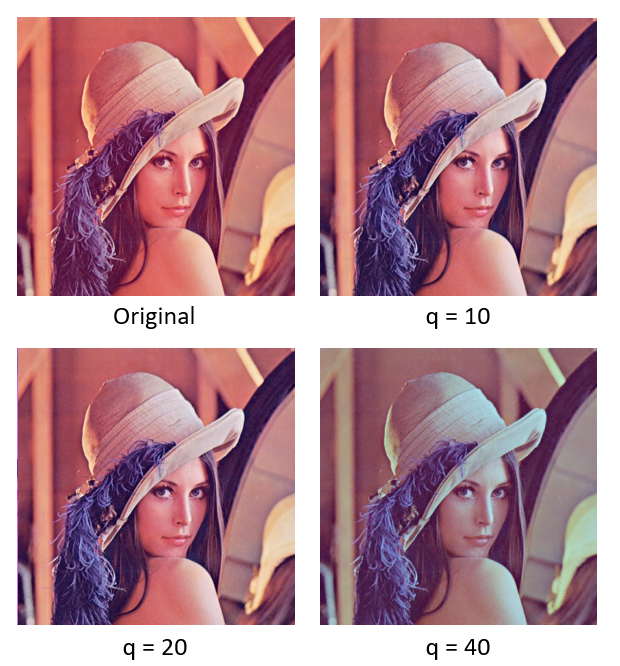
\includegraphics[scale=0.53]{Figures/fig27.png}
    \par \textbf {Hình 3.7} Kết quả nén ảnh lena.tif.
\end{center}
\begin{center}
    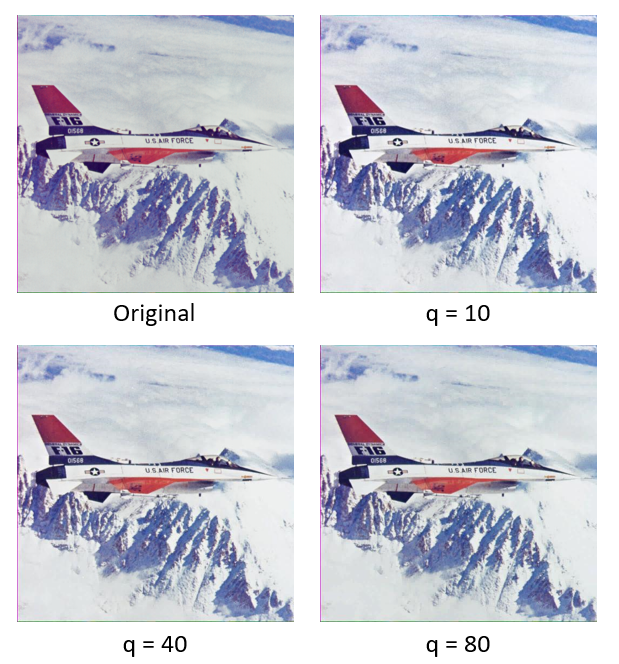
\includegraphics[scale=0.53]{Figures/fig26.png}
    \par \textbf {Hình 3.8} Kết quả nén ảnh airplane.png.
\end{center}
\begin{center}
    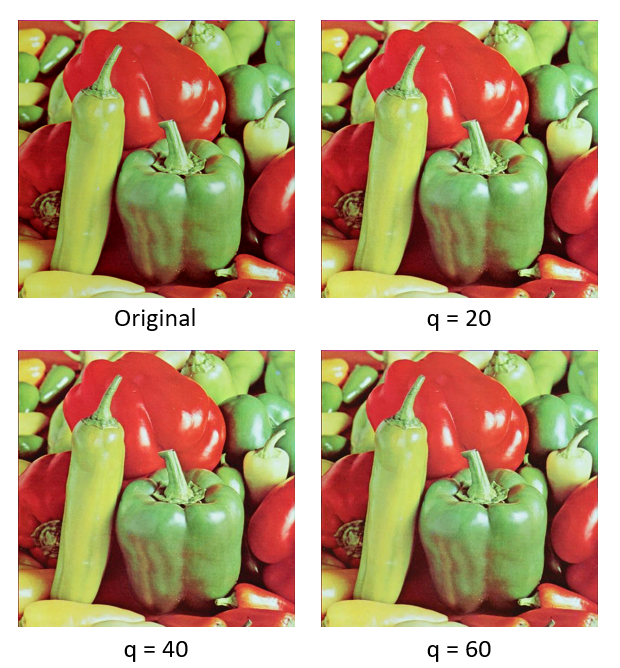
\includegraphics[scale=0.53]{Figures/fig28.png}
    \par \textbf {Hình 3.9} Kết quả nén ảnh pepers.png.
\end{center}
\begin{center}
    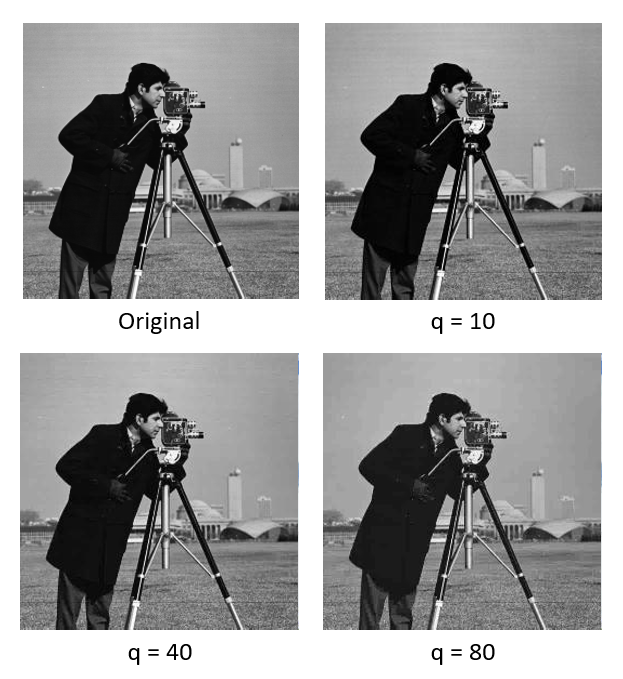
\includegraphics[scale=0.53]{Figures/fig25.png}
    \par \textbf {Hình 3.10} Kết quả nén ảnh cameraman.tif.
\end{center}
\begin{center}
    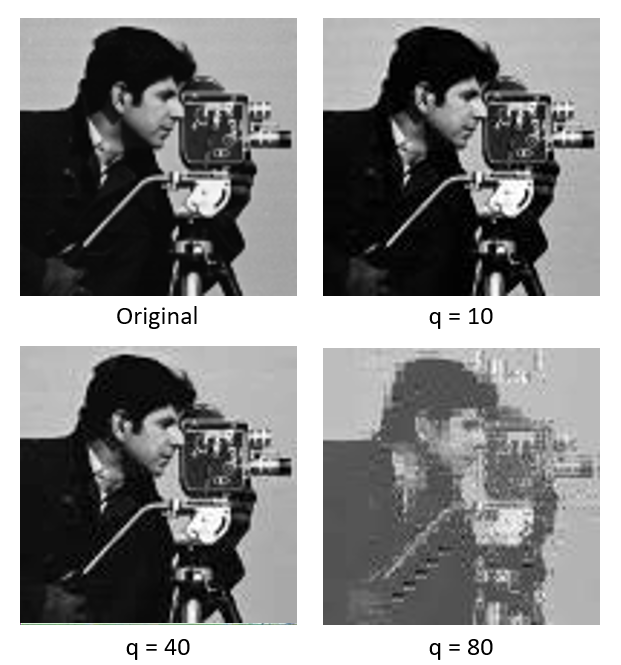
\includegraphics[scale=0.53]{Figures/fig29.png}
    \par \textbf {Hình 3.11} Kết quả nén một phần ảnh cameraman.tif kích thước 96x96.
\end{center}
% ---------------------------------------------------------------------------- %
% Chapter 4 - 
\chapter*{Lời Kết}\label{CH4}
\par Biến đổi Fourier có ứng dụng rất rộng rãi trong xử lý tín hiệu nói chung và xử lý ảnh số nói riêng, là tiền đề cho các toán tử phức tạp hiện tại. Các phương pháp lọc ảnh, nén ảnh, tăng cường ảnh,... hay các thao tác tiền xử lý ảnh trong các mô hình phức tạp dựa trên nền tảng toán học của biến đổi Fourier thu được hiệu quả cao khi làm việc với miền tần số. Bài báo cáo đã trình bày một cách tổng quát về nền tảng toán học, những ứng dụng cơ bản của biến đổi Fourier.

% ----------------------------------------------------------------------------
%
% List of Publications
%\addcontentsline{toc}{chapter}{List of Publications}
%\renewcommand{\bibname}{List of Publications}
%\renewcommand{\bibname}{Công bố khoa học}
%\begin{thebibliography}{1}


\end{thebibliography}
% ----------------------------------------------------------------------------%
% Bibliography
% ----------------------------------------------------------------------------
\renewcommand{\bibname}{Tài liệu tham khảo}
\begin{thebibliography}{1}
\bibitem{Pardela} A. Sokołowski, T. Pardela (2014). Application of Fourier Transforms in Classification of Medical Images. Advances in Intelligent Systems and Computing, 193-200.

\bibitem{Dogra} Ayush Dogra, Parvinder Bhalla (2014). Image Sharpening By Gaussian And Butterworth High Pass Filter. Department of ECE, Maharishi Markandeshwar University, Mullana, Ambala, India. Biomed Pharmacol J. 

\bibitem{Dogra} Chris Dogra, John Wiley, Sons (2007). Fundamental Principles of Optical Lithography: The Science of Microfabrication. 

\bibitem{Cooley} Cooley, James W.; Tukey, John W. (1965). An algorithm for the machine calculation of complex Fourier series. Math. Comput. 19 (90), 297–301.

\bibitem{Popa} Călin-Adrian Popa, Cosmin Cernăzanu-Glăvan (2018). Fourier Transform-Based Image Classification Using Complex-Valued Convolutional Neural Networks. International Symposium on Neural Networks (ISNN). Minsk, Belarus.

\bibitem{Daniel} Daniel B. Rowe, Andrew S. Nencka, Raymond G. Hoffmannb (2007). Signal and noise of Fourier reconstructed fMRI data. J Neurosci Methods, 361–369.

\bibitem{Escofet} Escofet, J., Millan, M.S. and Rallo, M. (2001). Applied Optics, Volume 40, Issue 34, pp. 6170-6176.

\bibitem{Granlund} G. H. Granlund (1972). Fourier processing for handwritten character recognition. IEEE Trans. Comput., vol. C-21, no. 3, pp. 195-201.

\bibitem{Harte} Harte, T.P. and Hanka R. (1997). Number Theoretic Transforms in Neural Network Image Classification.

\bibitem{Pharr} I. Pharr, Matt. II. Fernando, Randima (2005). Medical Image Reconstruction with the FFT. GPU gems 2. NVIDIA Corporation.

\bibitem{Levchenko} Levchenko, E.B., Myl’nikov, G.D., Timashev, A.N. and Turygin, A.Y. (1992). Neural network for image Fourier transform classification. Neuroinformatics and Neurocomputers, RNNS/IEEE Symposium. Vol. 1, pp 196-207.

\bibitem{Li} Li C.T., Wilson, R. (1995). Image Segmentation Using Multiresolution Fourier Transform. Department of Computer Science, University of Warwick.

\bibitem{Li} Li, J., Chen, L., \& Cai, Y. (2009). Dynamic Texture Segmentation Using 3-D Fourier Transform. 2009 Fifth International Conference on Image and Graphics. 

\bibitem{Li} Li-Wei Yang, Xiao-Feng Wang (2012). Leaf Image Recognition Using Fourier Transform Based on Ordered Sequence. ICIC 2012: Intelligent Computing Technology, pp 393-400.

\bibitem{Mohammed} Mohammed H. Rasheed, Omar M. Salih, Mohammed M. Siddeq, Marcos A.Rodrigues (2020). Image compression based on 2D Discrete Fourier Transform and matrix minimization algorithm. Elsevier Inc.

\bibitem{Efford} Nick Efford (2000). Digital Image Processing: A Practical Introduction Using JavaTM. Chapter 11: Morphological image processing. Pearson Education.

\bibitem{Paquet} Paquet, Eric, Rioux, Marc, Arsenault, Henri H. (1993). Range image segmentation using the Fourier transform. Optical Engineering 32(09), 2173-2180.

\bibitem{Rafael} Rafael C. Gonzalez, Richard E. Woods (2008). Digital Image Processing 3rd Edition.

\bibitem{Robert} Robert, P. (1980). Performance of the Discrete Fourier Transform Satellite Imagery Classification Technique. SYSTEMS AND APPLIED SCIENCES CORP RIVERDALE MD.

\bibitem{Shubing} Shubing Wang (2007). Applications of Fourier Transform to Imaging Analysis. 

\bibitem{Tang} Tang X. and Stewart W.K. (2000). Optical and Sonar Image Classification: Wavelet Packet Transform vs Fourier Transform. Computer Vision and Image Understanding, Volume 79, Number 1,
pp. 25-46(22).

\bibitem{Weisstein} Weisstein, Eric. Convolution Theorem. MathWorld.

\bibitem{Wu} Wu, H.S., Barba, J., Gil J. (1996). An iterative algorithm for cell segmentation using short-time Fourier transform. J Microsc. 184(Pt 2), 127-32.

\end{thebibliography}

%\ssp
%\renewcommand{\bibname}{References}
%\renewcommand{\bibname}{Tài liệu tham khảo}
%\bibliography{APPENDIX/References}
% ---------------------------------------------------------------------------- %
% Appendix 
%\newpage
%\appendix
% ---------------------------------------------------------------------------- % 
% Appendix A - 
% ---------------------------------------------------------------------------- %
%\input{..}
% ---------------------------------------------------------------------------- %
% Appendix B - 
% ---------------------------------------------------------------------------- %
%\input{..}
% ---------------------------------------------------------------------------- %
\end{document}
% ---------------------------------------------------------------------------- %